\if0
\section{Catalog of Symbols}
\label{app-sec:symbols}

\begin{table}[!ht]
  \centering
  \begin{tabular}{ll}
    \toprule
    Symbol & Description \\
    \midrule
    $\thb \in \mathbb{R}^D$ & Parameters \\
    $\ub$ & Nuisance variables \\
    $\yb \in \mathbb{R}^{D_{\yb}}$ & Simulator output \\
    $\data \in \mathbb{R}^{D_{\yb}}$ & Observation (if single) \\
    $\data_n$ & $n$-th observation (if multiple) \\
    $ \{ \data_n \}_{n=1}^N$ & Set of observations \\
    $\jac_{\thb}$ & Jacobian of the simulator at $\thb$ \\
    \midrule
    $p(\thb)$ & Prior distribution of the parameters \\
    $p(\ub)$ & Prior distribution of the nuisance variables \\
    $L_{\epsilon}(\thb)$ & ABC likelihood \\
    $L_{\epsilon}^n(\thb, \ub)$ & ABC likelihood for the $n$-th observation \\
    $p_{\epsilon}(\thb | \data)$ & ABC posterior (single observation) \\
    $p_{\epsilon}(\thb | \{ \data_n \}_{n=1}^N)$ & ABC posterior (multiple observations) \\
    $q(\thb)$ & Proposal distribution \\
    $q_i(\thb)$ & Proposal distribution for the $i$-th seed \\
    \midrule
    $g(\thb, \ub)$ & Simulator \\
    $d(\thb) = d(g(\thb, \ub), \data)$ & Distance function \\
    $d_i(\thb) = d(g(\thb, \ub_i), \data)$ & Distance function for the $i$-th seed \\
    \midrule
    $\accregioni$ & Acceptance region for the $i$-th seed \\
    % $d(\thb, \data)$ & Distance function \\
    % $d_i(\thb)$ & Distance function for the $i$-th seed \\
    % $\thb_i^*$ & Optimal point for the $i$-th seed \\
    % $\jac$ & Jacobian of the simulator \\
    % $w_i$ & Weight of the $i$-th seed \\
    % $q_i$ & Proposal distribution for the $i$-th seed \\
    % $V_i$ & Proposal area for the $i$-th seed \\
    % $\epsilon$ & Acceptance threshold for the optimal point \\
    % $\epsilon_2$ & Acceptance threshold for the proposal area \\
    % $\epsilon_3$ & Acceptance threshold for the samples \\
    \midrule
    $S$ & Number of seeds \\
    $M$ & Number of samples per proposal area \\
    $N$ & Number of observations \\
    $P$ & Number of samples at \rromc, Eq. (\ref{eq:romc_weight}) \\
    \midrule
    $n = 1, \ldots, N$ & Index of the observation \\
    $i = 1, \ldots, S$ & Index of the seed \\
    $j = 1, \ldots, M$ & Index of the sample \\
    \bottomrule
  \end{tabular}
  \caption{Catalog of symbols used in the paper.}
  \label{tab:symbols}
\end{table}
\fi

\section{Methods}
\label{app-sec:methods}

Throughout the paper we run experiments based on four methods: R2OMC (our proposal), NAIVE-ROMC~\citep[a straightforward use of the ROMC framework by][]{ikonomov2020robust}, Neural Posterior Estimation (NPE)~\citep{greenberg2019automatic}, Neural Likelihood Estimation (NLE)~\citep{papamakarios2019sequential}.

\paragraph{R2OMC.}

A detailed description of the method can be found in Algorithm~\ref{alg:r2omc}. 

In Step 2 of Algorithm~\ref{alg:r2omc}, i.e., computing the uninformative dimensions, we typically use around 50 samples from the distribution \(p(u)\) and another 50 samples from \(p(\thb)\), with the parameter \(\tau\) set to machine precision, i.e., \(\tau \approx 0\). Similar results can be obtained with fewer samples, such as 10 or 20.

For Step 3, i.e., computing the optimal points \(\thb_{i,n}^*\), we use the Adam optimizer, with a learning rate between 0.01 and 0.2, depending on the specific problem. Our default choice is 0.1. The number of optimization steps varies between 100 and 400, with 50 as the  default. The distance function \(d(\thb)\) is defined as the squared Euclidean distance between the simulator output and the observation, i.e., \(d(\thb) = \|\yb - \data_n\|^2_2\).
The number of seeds \(S\) used ranges from 500 to 5000, with 1000 as the default. The number of seeds corresponds to the simulation budget; for example, if a budget of 10,000 runs is available, we use (at most) 10,000 seeds. Typically, we select 80\% of the seeds based on the best \(d_i^n(\thb_{i,n}^*)\). However, the percentage of accepted seeds can vary between 50\% and 100\%, depending on the absolute values of \(d_i^n(\thb_{i,n}^*)\) for \(i = 1, \dots, S\).

For Step 5, i.e., constructing the hyperboxes, we use Algorithm~\ref{alg:region_construction}. We normally set \(\epsilon\) to be twice the distance of the `worst' accepted seed, i.e., \(\epsilon = 2 \max_i d_i^n(\thb_{i,n}^*)\), where \(i\) is an index over the accepted seeds. Alternatively, \(\epsilon\) can be set to a fixed value such as $0.1$. The typical settings for step size, number of steps, and refinements are \(\eta = 0.1\), \(L = 100\), and \(R = 1\), respectively.

For Step 7, i.e., sampling from the proposal distribution, we generate between 1000 and 100,000 candidate samples, with the default being 5000. From these candidates, we select 1000 via weighted sampling.
For computing the weights, $\{w_p\}_{p=1}^{P}$, we set $\epsilon$ to a value about twice the distance of the `worst' accepted seed, i.e., $\epsilon = 2 \max_{i,n} d_i^n(\thb_{i,n}^*)$. However, this can vary depending on the problem, and by testing different values.

Finally, we keep 1000 posterior samples, which are used to compute the \texttt{C2ST} score using another 1000 samples drawn from the true posterior.

\begin{algorithm}[!ht]
  \caption{Hyperbox Computation \newline
    \textit{Input:} Optimal point \(\thb^*\), distance function \(d(\thb)\), Jacobian \(\jac\) at \(\thb^*\) \newline
    \textit{Parameters:} Step size \(\eta\), number of refinements \(R\), number of steps \(L\), distance threshold \(\epsilon\)}
  \label{alg:region_construction}
  \begin{algorithmic}[1]
    \State Compute eigenvectors \(\vb_d\) of \(\jac^T\jac\) {\scriptsize (\(d = 1,\ldots,D)\)}
    \For{\(d = 1\) to \(D\)}
      \State Initialize endpoint \(\Tilde{\thb} \gets \thb^*\)
      \State Set refinement counter \(r \gets 0\)
      \Repeat{}
        \State Set step counter \(l \gets 0\)
        \Repeat{}
          \State Increment step counter \(l \gets l + 1\)
          \State Update \(\Tilde{\thb} \gets \Tilde{\thb} + \eta \vb_d\)
        \Until{\(d(\thb) > \epsilon\) or \(l = L\)}
        \State Move back one step \(\Tilde{\thb} \gets \Tilde{\thb} - \eta \vb_d\)
        \State Halve the step size \(\eta \gets \eta/2\)
        \State Increment refinement counter \(r \gets r + 1\)
      \Until{\(r = R\)}
      \State Set \(\Tilde{\thb}\) as the endpoint
      \State Repeat steps 3-15 for \(\vb_d = - \vb_d\) and set \(\Tilde{\thb}\) as the negative endpoint
    \EndFor
    \State Define a uniform distribution \(q\) over the hyperbox
    \State \Return \(q\)
  \end{algorithmic}
\end{algorithm}


\paragraph{NAIVE-ROMC.}

We use the Algorithm presented as ROMC in~\cite{ikonomov2020robust}. The characterization NAIVE indicates the use of a naive distance function in case of multiple observations. As described in the main paper, in case of $N$ observations, we concatenate them in a single vector $\data = (\mathbf{y}^{o, (1)}, \ldots, \mathbf{y}^{o, (N)})$, then, run the simulator $N$ times, concatenate the ouputs, $\yb = (\yb^{(1)}, \ldots, \yb^{(N)})$ and set the distance to be the squared Euclidean distance between the two vectors, $d(\thb) = ||\yb-\data||_2^2$.
Although using this approach for defining $d(\thb)$ has disadvantages, that is why we name it `NAIVE', there is no other (simple) approach that leads to a better posterior approximation, under multiple observations.

\nromc~is practically the same as \rromc~(Algorithm~\ref{alg:r2omc} of the main text), if (a) we omit Step 2, i.e., computing the uninformative dimensions and (b) set $N=1$.
This is why \nromc~and \rromc~have a similar \texttt{C2ST} score in problems without distractors and with a single observation.
In case of multiple observations, we use as $\yb$ and $\data$, the concatenated vectors as described above.
For \nromc, we use a $\texttt{JAX}$-based implementation that is similar to the one we use for \rromc. The reason for not using its existing implementation~\citep{gkolemis2023extendable} of the ELFI package~\citep{elfipackage} is that it does not use gradients, so it cannot scale to high dimensions.
The hyperparameters used in \nromc~are similar to \rromc, as described above. 

\paragraph{NPE}

% In all cases, we use a simulation budget of up to 10,000 simulator executions. SNPE and NLE are chosen as representatives of the Neural Density Estimation (NDE) family. We opt for the sequential version of NPE (i.e., SNPE) due to its slightly better performance at a comparable computational cost. In contrast, we use the single-round version of NLE, as its sequential counterpart (SNLE) incurred significantly higher computational costs with a fractional imporverment in the performance.
% Overall, in our experiments with a simulation budget of 10,000 runs, we observed no substantial difference between the sequential and non-sequential versions of the methods and since the focus of this paper is not on this comparison, we selected SNPE and NLE for convenience.


As Neural Posterior Estimation (NPE) we use the one denoted as as SNPE\_C in the SBI benchmark~\citep{lueckmann2021benchmarking}, which is a method proposed by~\citet{greenberg2019automatic}.
SNPE\_C estimates the posterior by training a neural network \( F(\yb, \phi) \) to approximate \( p(\thb|\yb) \) using a density estimator \( q_F(\yb, \phi)(\thb) \). For further details, see~\citep{greenberg2019automatic}.

We use the \texttt{Pytorch} implementation provided by the SBI package, using mostly the default parameters. As density estimator we use the a neural network with 50 hidden units,
\texttt{sbi.utils.get\_nn\_models.posterior\_nn()} with parameters 
\texttt{model=`nsf'},
\texttt{hidden\_features=50},
\texttt{z\_score\_x=`independent'}, and
\texttt{z\_score\_x=`independent'}.
During training, we use $10$ atoms, a batch size of $1000$ (or the whole dataset) and a maximum number of $500$ epochs.

We use a simulation budget of $10,000$ simulator executions, which means that we train the density estimator on $10,000$ samples.
We normally use $2$ training rounds, each with $5000$ training samples: the first set of $5000$ is drawn from the prior, while the second set is sampled from the approximate posterior learned after the first round. Occasionally, if the initial $5000$ samples do not yield a reliable approximation and conditioning on $\data$ leads to instabilities, we use a single round of $10000$ samples.

In cases with multiple observations, since \NPE~cannot handle them separately, we follow the same approach as in \nromc (see above); we concatenate the observations and the outputs to one vector each.

\paragraph{NLE}

As NLE we use the method proposed by~\cite{papamakarios2019sequential}.
NLE approximates the likelihood \( p(\data|\theta) \) using neural density estimation. The process involves generating a dataset \( D = \{(\thb_k, \yb_k)\}_{k=1}^K \) by sampling \( \thb_k \sim p(\thb) \) and simulating \( \yb_k \sim p(\yb|\thb_k) \). A conditional neural density estimator \( q_\psi(\yb|\thb) \) is then trained to model the likelihood.

Once trained, samples from the posterior \( \hat{p}(\thb|\data) \propto q_\psi(\data|\thb) p(\thb) \) are obtained using MCMC.
For density estimation, we use the default SBI settings, i.e., a Masked Autoregressive Flow (MAF) with five flow transforms and 50 hidden units per block. For MCMC, 250 warm-up steps and posterior samples are obtained with thinning.

We use a simulation budget of $10,000$ simulator executions, which means that we train the density estimator on $10,000$ samples. We always use a single training round.
\NLE~can handle multiple observations; we simply pass a \texttt{numpy} array of shape: \texttt{(N,D)}, where $N$ is the number of observations and $D$ their dimensionality. Internally, \NLE~evaluates each observation using the neural density estimator $ q_\psi(\yb|\thb) $ and multiplies them to estimate the joint likelihood and then uses MCMC to sample from the posterior.

\clearpage

\section{Introductory Example}
\label{app-sec:intro-example}

\paragraph{Notation.}

We use $\mathcal{N}(\mathbf{y}; \thb, \Sigma)$ to denote the probability density function (pdf) of a Gaussian random variable $\yb$, while $\mathcal{N}(\boldsymbol{\theta}, \Sigma)$ denotes the random variable itself. Typically, $\mathcal{N}(\mathbf{y}; \thb, \Sigma)$ is used when deriving expressions, whereas $\mathcal{N}(\thb, \Sigma)$ is used to indicate sampling, such as in $\mathbf{y} \sim \mathcal{N}(\thb, \Sigma)$. We use $\mathcal{U}(\mathbf{a}, \mathbf{b})$ to denote a multivariate random variable that is uniformly distributed on the hypercube defined by vector $\mathbf{a}$ with the lower boundaries and the vector $\mathbf{b}$ with the upper boundaries. The dimensions are typically clear from the context if not explicitly stated. Bold indicates a vector, e.g., $\thb \in \mathbb{R}^D$.

\paragraph{Setup.}

We provide further details about the introductory example shown in Figure~\ref{fig:concept_example}.
The introductory example consists of five different versions:
(1) Simple,
(2) High-dimensional,
(3) Distractor,
(4) Multiple observations, and
(5) Combined.

The simulator of the Simple (1), High-dimensional (2) and Multiple observations (4) versions is:
\begin{equation}
  \label{eq:intro-simulator}
  \mathbf{y} \sim \frac{1}{2} \left( \mathcal{N}(\boldsymbol{\theta}, \mathbf{I}) + \mathcal{N}(-\boldsymbol{\theta}, \mathbf{I}) \right)
\end{equation}
%
At the Distractor (3) and the Combined (5) versions, we add $D_{\text{dist}} = 10$ distractor dimensions to the output, so the simulator becomes:
\begin{equation}
  \label{eq:intro-simulator-distractor}
  (\mathbf{y}^{(1)}, \mathbf{y}^{(2)}), \quad \mathbf{y}^{(1)} \sim \frac{1}{2} \left( \mathcal{N}(\boldsymbol{\theta}, \mathbf{I}) + \mathcal{N}(-\boldsymbol{\theta}, \mathbf{I}) \right), \quad \mathbf{y}^{(2)} \sim \mathcal{N}(\boldsymbol{\mu}, 100 \mathbf{I}),
\end{equation}
%
where $\boldsymbol{\mu} \sim \mathcal{U}(-\mathbf{10}, \mathbf{10})$.
In all cases the prior is given by \(p(\boldsymbol{\theta}) = \mathcal{U}(\mathbf{-15}, \mathbf{15}) \).

\subsection{Simple Case}

The simulator is the one in (\ref{eq:intro-simulator}) with $D = 5$ and
the observation is $\data = (5, \ldots, 5) + \epsilon$ where $\data \in \mathbb{R}^5$.
The ground truth posterior for $\data = (5, \ldots, 5)$ is given by:
\begin{align}
  p(\thb | \data)
  &\propto p(\thb) p(\data | \boldsymbol{\theta}) \\
  &\propto p(\thb) ( \mathcal{N}(\data; \boldsymbol{\theta}, \mathbf{I}) + \mathcal{N}(\data; -\boldsymbol{\theta}, \mathbf{I}) ) \label{eq:intro-simple-1} \\
  &\propto p(\thb) ( \mathcal{N}(\boldsymbol{\theta}; \data, \mathbf{I}) + \mathcal{N}(\boldsymbol{\theta}; -\data, \mathbf{I}) ) \label{eq:intro-simple-2} \\
  &\propto
    \begin{cases}
      \mathcal{N}(\boldsymbol{\theta}; \mathbf{5}, \mathbf{I}) + \mathcal{N}(\boldsymbol{\theta}; -\mathbf{5}, \mathbf{I}), & \text{if } \boldsymbol{\theta} \in [-15, 15]^5, \\
      0, & \text{otherwise}.
    \end{cases}
    \label{eq:intro-simple}
\end{align}
%
From~(\ref{eq:intro-simple-1}) to~(\ref{eq:intro-simple-2}), we apply the property: $\mathcal{N}(\yb; - \thb, \Sigma) = \mathcal{N}(\thb; - \yb , \Sigma)$.

\subsection{High-dimensional Case}

The simulator is the one in (\ref{eq:intro-simulator}) with $D = 20$ and
the observation is $\data = (5, \ldots, 5) + \epsilon$ where $\data \in \mathbb{R}^{20}$.
The derivation of (\ref{eq:intro-simple}) holds irrespectively of the dimensionality, so the ground truth posterior for $\data = (5, \ldots, 5)$ is:
%
\begin{equation}
  p(\boldsymbol{\theta} | \data) \propto
  \begin{cases}
    \mathcal{N}(\boldsymbol{\theta}; \mathbf{5}, \mathbf{I}) + \mathcal{N}(\boldsymbol{\theta}; -\mathbf{5}, \mathbf{I}), & \text{if } \boldsymbol{\theta} \in [-15, 15]^{20}, \\
    0, & \text{otherwise}.
  \end{cases}
  \label{eq:intro-highdim}
\end{equation}
%
\subsection{Distractor Case}

The simulator is the one in (\ref{eq:intro-simulator-distractor}) with $D = 5$ and $D_{\text{dist}} = 10$, leading to an output dimensionality of $D_y + D_{\text{dist}} = 15$.
The observation is $\data = (\mathbf{y}^{o,(1)}, \mathbf{y}^{o,(2)})$,
where
$\mathbf{y}^{o,(1)} = (5, \ldots, 5) + \epsilon$
and
$\mathbf{y}^{o,(2)} = (0, \ldots, 0) + \epsilon$.
Below, we show that the ground truth posterior is equivalent to the simple case (\ref{eq:intro-simple}), as the distractor dimensions do not affect the posterior:
%
\begin{align}
  p(\boldsymbol{\theta} | \data)
  &\propto p(\boldsymbol{\theta}) p(\data | \boldsymbol{\theta}) \\
  &\propto p(\boldsymbol{\theta}) p((\mathbf{y}^{o,(1)}, \mathbf{y}^{o,(2)}) | \boldsymbol{\theta}) \label{eq:intro-distractors-1} \\
  &\propto p(\boldsymbol{\theta}) p(\mathbf{y}^{o,(1)} | \boldsymbol{\theta}) p(\mathbf{y}^{o,(2)} | \boldsymbol{\theta}) \label{eq:intro-distractors-2} \\
  &\propto p(\boldsymbol{\theta}) p(\mathbf{y}^{o,(1)} | \boldsymbol{\theta}) p(\mathbf{y}^{o,(2)}) \label{eq:intro-distractors-3} \\
  &\propto p(\boldsymbol{\theta}) p(\mathbf{y}^{o,(1)} | \boldsymbol{\theta}) \\
  &\propto
  \begin{cases}
    \mathcal{N}(\boldsymbol{\theta}; \mathbf{5}, \mathbf{I}) + \mathcal{N}(\boldsymbol{\theta}; -\mathbf{5}, \mathbf{I}), & \text{if } \boldsymbol{\theta} \in [-15, 15]^5, \\
    0, & \text{otherwise}.
  \end{cases}
  \label{eq:intro-distractors}
\end{align}
%
From (\ref{eq:intro-distractors-1}) to (\ref{eq:intro-distractors-2}), we use that $\mathbf{y}^{o,(1)}$ is independent of $\mathbf{y}^{o,(2)}$ and
from (\ref{eq:intro-distractors-2}) to (\ref{eq:intro-distractors-3}), that $\mathbf{y}^{o,(2)}$ is independent of $\thb$.

\subsection{Multiple Observations Case}
The simulator is the one in (\ref{eq:intro-simulator}) with $D = 5$ and
the set of $N=4$ iid observations is $\{\data_n\}_n^N$ where $\data_n = (5, \ldots, 5) + \epsilon$ for $n = 1, 2$ and $\data_n = (-5, \ldots, -5) + \epsilon$ for $n = 3, 4$.
We will derive the ground truth posterior for the general case of $N$ observations, where $\data_n = (5, \ldots, 5) + \epsilon$ for $n \in \{1, \ldots, N/2\}$ and $\data_n = (-5, \ldots, -5) + \epsilon$ for $n \in \{N/2+1, \ldots, N\}$.
%
\begin{align}
  p(\thb|\{\data_k\})
  &\propto p(\thb) \prod_n^{N} p(\data_n | \thb) \\
  &\propto p(\thb) \prod_{n=1}^{N/2} p(\data_n | \thb) \prod_{n=N/2+1}^{N} p(\data_n | \thb) \label{eq:intro-multiple-1} \\
  &\propto p(\thb) \prod_{n=1}^{N/2} (\mathcal{N}(\mathbf{5}; \thb, \mathbf{I}) + \mathcal{N}(-\mathbf{5}; \thb, \mathbf{I})) \prod_{n=N/2+1}^{N} (\mathcal{N}(-\mathbf{5}; \thb, \mathbf{I}) + \mathcal{N}(\mathbf{5}; \thb, \mathbf{I})) \label{eq:intro-multiple-2} \\
  &\propto p(\thb) \prod_{n=1}^{N} (\mathcal{N}(\mathbf{5}; \thb, \mathbf{I}) + \mathcal{N}(-\mathbf{5}; \thb, \mathbf{I})) \label{eq:intro-multiple-3} \\
  &\propto p(\thb) \prod_{n=1}^{N} (\mathcal{N}(\thb; \mathbf{5}, \mathbf{I}) + \mathcal{N}(\thb; - \mathbf{5}, \mathbf{I})) \label{eq:intro-multiple-4} \\
  &\appropto p(\thb) ( \mathcal{N}(\thb; \mathbf{5}, \mathbf{I}) )^N + ( \mathcal{N}( \thb; - \mathbf{5}, \mathbf{I}) )^N \label{eq:intro-multiple-5} \\
  &\appropto p(\thb) ( \mathcal{N}(\thb; \mathbf{5}, \frac{1}{N}\mathbf{I} ) + \mathcal{N}(\thb; - \mathbf{5}, \frac{1}{N}\mathbf{I} ) ) \label{eq:intro-multiple-6} \\
  &\appropto
  \begin{cases}
    \mathcal{N}(\thb; \mathbf{5}, \frac{1}{N}\mathbf{I} ) + \mathcal{N}(\thb; - \mathbf{5}, \frac{1}{N}\mathbf{I} ), & \text{if } \thb \in [-15, 15]^5, \\
    0, & \text{otherwise}.
  \end{cases}
  \label{eq:intro-multiple}
\end{align}
%
From (\ref{eq:intro-multiple-1}) to (\ref{eq:intro-multiple-2}), we simply plug in the corresponding observations.
From (\ref{eq:intro-multiple-3}) to (\ref{eq:intro-multiple-4}), we apply the property: $\mathcal{N}(\yb; - \thb, \Sigma) = \mathcal{N}(\thb; - \yb , \Sigma)$.
From (\ref{eq:intro-multiple-4}) to (\ref{eq:intro-multiple-5}), we use that the terms that include the product
$\mathcal{N}(\thb; \mathbf{5}, \mathbf{I})\mathcal{N}(\thb; - \mathbf{5}, \mathbf{I})$ have a much smaller magnitude than the two terms
$\mathcal{N}(\thb; \mathbf{5}, \mathbf{I})^N$ and $\mathcal{N}(\thb; - \mathbf{5}, \mathbf{I})^N$. Therefore, we keep only the latter in (\ref{eq:intro-multiple-5}).
From (\ref{eq:intro-multiple-5}) to (\ref{eq:intro-multiple-6}), we use the property: $\mathcal{N}(\thb; \mub, \Sigma)^N = \mathcal{N}(\thb; \mub, \frac{1}{N}\Sigma)$.

\subsection{Combined Case}
The simulator is the one in~(\ref{eq:intro-simulator-distractor}) with $D = 20$ and $D_{\text{dist}} = 10$, leading to an output dimensionality of $D_y + D_{\text{dist}} = 30$.
The set of $N=4$ iid observations is $\{\data_n\}_n^N$ where $\data_n = (\mathbf{y}^{o,(1)}, \mathbf{y}^{o,(2)})$, with $\mathbf{y}^{o,(1)}$ equal $(5, \ldots, 5) + \epsilon$ for $n \in \{1, \ldots, N/2\}$ and $(-5, \ldots, -5) + \epsilon$ for $n \in \{N/2+1, \ldots, N\}$ and $\mathbf{y}^{o,(2)}$ equal $(0, \ldots, 0) + \epsilon$ for all $n$.

Using the properties of the previous cases we obtain the ground truth posterior, which is the same as in the multiple observations case (\ref{eq:intro-multiple}) for $D = 20$:
%
\begin{align}
  p(\thb|\{\data_k\})
  &\propto p(\thb) \prod_n^{N} p(\data_n | \thb) \label{eq:intro-combined-1} \\
  &\propto p(\thb) \prod_{n=1}^{N} p((\mathbf{y}^{o,(1)}, \mathbf{y}^{o,(2)}) | \thb) \label{eq:intro-combined-2} \\
  &\propto p(\thb) \prod_{n=1}^N p(\mathbf{y}^{o,(1)} | \thb) p(\mathbf{y}^{o,(2)} | \thb) \label{eq:intro-combined-3} \\
  &\propto p(\thb) \prod_{n=1}^N p(\mathbf{y}^{o,(1)} | \thb) p(\mathbf{y}^{o,(2)}) \label{eq:intro-combined-4} \\
  &\propto p(\thb) \prod_{n=1}^N p(\mathbf{y}^{o,(1)} | \thb) \label{eq:intro-combined-5}
  \end{align}
From (\ref{eq:intro-combined-2}) to (\ref{eq:intro-combined-3}), we use that the observations are independent and
from (\ref{eq:intro-combined-3}) to (\ref{eq:intro-combined-4}) that $\mathbf{y}^{o,(2)}$ is independent of $\thb$.
Using the derivation of the multiple observations case (\ref{eq:intro-multiple}) gives
  \begin{align}
  p(\thb|\{\data_k\})
  &\appropto
  \begin{cases}
    \mathcal{N}(\thb; - \mathbf{5}, \frac{1}{N}\mathbf{I} ) + \mathcal{N}(\thb; \mathbf{5}, \frac{1}{N}\mathbf{I} ), & \text{if } \thb \in [-15, 15]^{20}, \\
    0, & \text{otherwise}.
  \end{cases}
  \label{eq:intro-combined}
\end{align}


\subsection{Results}

\paragraph{Setup.}
For \nromc and \rromc, a maximum of $S=5000$ seeds was used, corresponding to approximately 5000 independent simulator calls, which is (approximately) a simulation budget of 5000.
\NLE~and \NPE~were trained with a simulation budget of 10000 samples.
For \NPE, we used $R=2$ rounds with $5000$ samples each, while for NLE, we used a single round of $10000$ samples.
The default settings from the SBI library~\cite{lueckmann2021benchmarking} were utilized for both, with a training batch size of $1000$ and a maximum of $300$ training epochs.

\paragraph{Conclusions.}
The results of the introductory example are presented in Figure~\ref{fig:concept_example} in the main text.
In the simple scenario, all methods provide a reasonably accurate approximation of the ground truth posterior.
In the high-dimensional case, both \NPE~and \NLE~encounter difficulties, indicating that high-dimensional problems are challenging for these methods even when the simulator is relatively simple.
In contrast, \nromc~and~\rromc~yield a good approximation of the ground truth posterior, demonstrating their robustness in high-dimensional settings.
Note that in the simple scenario, \nromc~and~\rromc~are equivalent, since there are no distractors and only one observation.
In the distractors scenario, \NPE~struggles, \NLE~is more robust than \NPE, but still faces challenges in providing an accurate approximation, while \nromc~struggles.
\rromc~provides a good approximation of the ground truth posterior.
In the multiple observations scenario, only \NLE~and \rromc~succeed in generating a reliable approximation of the ground truth posterior.
Finally, in the combined scenario, only \rromc~delivers a satisfactory approximation of the ground truth posterior.


\clearpage
\section{Additional information on the experiments}
\label{app-sec:experiments}

We here provide some additional information on the experiments presented in the main text.

\subsection{MoG Benchmark - High Dimensional Simulators}

\subsubsection{Base simulator - without distractors}

\begin{tabular}{@{}ll@{}}
  \textbf{Prior} & $\thb \sim \mathcal{U}(-\mathbf{15}, \mathbf{15})$ \\ [5pt]
  \textbf{Simulator} & $\yb \sim \mathcal{N}(\thb, \sigma^2 \mathbf{I}) \label{eq:mog_base}$, with $\sigma^2 = 1.5^2$ \\ [5pt]
  \textbf{Dimensionality} & $\thb \in \mathbb{R}^{D}$, $\yb \in \mathbb{R}^{D}$ \\ [5pt]
  \textbf{Observation} & $\data = (5, \ldots, 5) + \epsilon$ where $\data \in \mathbb{R}^D$ \\ [5pt]
  \textbf{Posterior} & $ p(\thb | \data) \propto
                                    \begin{cases}
                                      \mathcal{N}(\thb; \mathbf{5}, \sigma^2 \mathbf{I}), & \text{if } \thb \in [-15, 15]^D, \\
                                      0, & \text{otherwise}.
                                    \end{cases} $ \\ [5pt]
\end{tabular}

\textbf{Proof of the posterior:}
%
\begin{align}
  p(\thb | \data) &\propto p(\thb) p(\data | \thb) \label{eq:mog_base_posterior-1} \\
                  &\propto p(\thb) \mathcal{N}(\data; \thb, \sigma^2 \mathbf{I}) \label{eq:mog_base_posterior-2} \\
                  &\propto p(\thb) \mathcal{N}(\thb; \data, \sigma^2 \mathbf{I}) \label{eq:mog_base_posterior-3} \\
                  &\propto
                    \begin{cases}
                      \mathcal{N}(\thb; \mathbf{5}, \sigma^2 \mathbf{I}), & \text{if } \thb \in [-15, 15]^D, \\
                      0, & \text{otherwise}.
                    \end{cases} \label{eq:mog_base_posterior}
\end{align}

From~(\ref{eq:mog_base_posterior-2}) to~(\ref{eq:mog_base_posterior-3}), we apply the property: $\mathcal{N}(\yb; - \thb, \Sigma) = \mathcal{N}(\thb; - \yb , \Sigma)$.


\subsubsection{Base simulator - with distractors}

\begin{tabular}{@{}ll@{}}
  \textbf{Prior} & $\thb \sim \mathcal{U}(-\mathbf{15}, \mathbf{15})$ \\ [5pt]
  \textbf{Simulator} & $\yb = (\mathbf{y^{(1)}}, \mathbf{y^{(2)}})$, \\ [5pt]
  & $\mathbf{y^{(1)}} \sim \mathcal{N}(\thb, \sigma^2 \mathbf{I})$, $\sigma^2=1.5^2$, \\ [5pt]
  & $\mathbf{y^{(2)}} \sim \mathcal{N}(\boldsymbol{\mu}, 100 \mathbf{I})$, $\boldsymbol{\mu} \sim \mathcal{U}(-\mathbf{10}, \mathbf{10})$ \\ [5pt]
  \textbf{Dimensionality} & $\thb \in \mathbb{R}^D,  \yb \in \mathbb{R}^{D + 100}$, $\yb^{(1)} \in \mathbb{R}^{D}$, $\yb^{(2)} \in \mathbb{R}^{100}$\\ [5pt]
  \textbf{Observation} & $\data = (\mathbf{y^{o, (1)}}, \mathbf{y^{o, (2)}})$, where $\mathbf{y^{o, (1)}} = (5, \ldots, 5) + \epsilon$ and $\mathbf{y^{o, (2)}} = (0, \ldots, 0) + \epsilon$ \\ [5pt]
  \textbf{Posterior} & $ p(\thb | \data) \propto
                                    \begin{cases}
                                      \mathcal{N}(\thb; \mathbf{5}, \sigma^2 \mathbf{I}), & \text{if } \thb \in [-15, 15]^D, \\
                                      0, & \text{otherwise}.
                                    \end{cases} $ \\ [5pt]
\end{tabular}

The ground truth posterior is the same as in~(\ref{eq:mog_base_posterior}), as the distractors do not affect the posterior, see (\ref{eq:intro-distractors}).

\subsubsection{MoG simulator - without distractors}

\begin{tabular}{@{}ll@{}}
  \textbf{Prior} & $\thb \sim \mathcal{U}(-\mathbf{15}, \mathbf{15})$ \\ [5pt]
  \textbf{Simulator} & $\yb \sim \frac{1}{2} \left( \mathcal{N}(\thb, \sigma_1^2\mathbf{I}) + \mathcal{N}(-\thb, \sigma_2^2\mathbf{I}) \right)$, $\sigma_1^2=0.1$, $\sigma_2^2=1$ \\ [5pt]
  \textbf{Dimensionality} & $\thb \in \mathbb{R}^{D}$, $\yb \in \mathbb{R}^{D}$ \\ [5pt]
  \textbf{Observation} & $\data = (5, \ldots, 5) + \epsilon$ where $\data \in \mathbb{R}^D$ \\ [5pt]
  \textbf{Posterior} & $ p(\thb | \data) \propto
                                    \begin{cases}
                                      \mathcal{N}(\thb; \mathbf{5}, \sigma_1^2 \mathbf{I}) + \mathcal{N}(\thb; -\mathbf{5}, \sigma_2^2 \mathbf{I}), & \text{if } \thb \in [-15, 15]^D, \\
                                      0, & \text{otherwise}.
                                    \end{cases} $ \\ [5pt]
\end{tabular}

The MoG simulator is the same as in the introductory example, so the proof is equivalent to Section~\ref{app-sec:intro-example}.

\subsubsection{MoG simulator - with distractors}

\begin{tabular}{@{}ll@{}}
  \textbf{Prior} & $\thb \sim \mathcal{U}(-\mathbf{15}, \mathbf{15})$ \\ [5pt]
  \textbf{Simulator} & $\yb=(\mathbf{y^{(1)}}, \mathbf{y^{(2)}})$,\\[5pt]
  &$\mathbf{y^{(1)}} \sim \frac{1}{2} \left ( \mathcal{N}(\thb, \sigma_1^2 \mathbf{I}) + \mathcal{N}(-\thb, \sigma_2^2 \mathbf{I}) \right )$, $\sigma_1^2=0.1$, $\sigma_2^2=1$,\\[5pt]
  &$\mathbf{y^{(2)}} \sim \mathcal{N}(\boldsymbol{\mu}, 100 \mathbf{I})$, $\boldsymbol{\mu} \sim \mathcal{U}(\mathbf{-10}, \mathbf{10})$ \\ [5pt]
  \textbf{Dimensionality} & $\thb \in \mathbb{R}^{D}$, $\yb \in \mathbb{R}^{D + 100}$, $\yb^{(1)} \in \mathbb{R}^{D}$, $\yb^{(2)} \in \mathbb{R}^{100}$ \\ [5pt]
  \textbf{Observation} & $\data = (\mathbf{y^{o, (1)}}, \mathbf{y^{o, (2)}})$, where $\mathbf{y^{o, (1)}} = (5, \ldots, 5) + \epsilon$ and $\mathbf{y^{o, (2)}} = (0, \ldots, 0) + \epsilon$ \\ [5pt]
  \textbf{Posterior} & $ p(\thb | \data) \propto
                                    \begin{cases}
                                      \mathcal{N}(\thb; \mathbf{5}, \sigma_1^2 \mathbf{I}) + \mathcal{N}(\thb; -\mathbf{5}, \sigma_2^2 \mathbf{I}), & \text{if } \thb \in [-15, 15]^D, \\
                                      0, & \text{otherwise}.
                                    \end{cases} $ \\ [5pt]
\end{tabular}

The MoG simulator is the same as in the introductory example, so the proof is equivalent to Section~\ref{app-sec:intro-example}.

\subsection{MoG Benchmark - Multiple Observations}

\subsubsection{Base simulator}

\begin{tabular}{@{}ll@{}}
  \textbf{Prior} & $\thb \sim \mathcal{U}(-\mathbf{15}, \mathbf{15})$ \\ [5pt]
  \textbf{Simulator} & $\yb \sim \mathcal{N}(\yb; \thb, \sigma^2 \mathbf{I})$, $\sigma^2=1$ \\ [5pt]
  \textbf{Dimensionality} & $\thb \in \mathbb{R}^{D}$, $\yb \in \mathbb{R}^{D}$ \\ [5pt]
  \textbf{Observations} & $\{\data_n\}_n^N$ where $\data_n = (5, \ldots, 5) + \epsilon$ for $n \in \{1, \ldots, 4\}$ \\ [5pt]
  \textbf{Posterior} & $ p(\thb | \data) \propto
                                    \begin{cases}
                                      \mathcal{N}(\thb; \mathbf{5}, \frac{1}{N}\sigma^2 \mathbf{I}), & \text{if } \thb \in [-15, 15]^D, \\
                                      0, & \text{otherwise}.
                                    \end{cases} $ \\ [5pt]
\end{tabular}

\textbf{Proof of the posterior:}
\begin{align}
  p(\thb|\{\data_n\})
  &\propto p(\thb) \prod_n^{N} p(\data_n | \thb) \label{eq:mog_mult_obs-1} \\
  &\propto p(\thb) \prod_{n=1}^{N} \mathcal{N}(\data_n; \thb, \sigma^2 \mathbf{I}) \label{eq:mog_mult_obs-2} \\
  &\propto p(\thb) \prod_{n=1}^{N} \mathcal{N}(\thb; \data_n, \sigma^2 \mathbf{I}) \label{eq:mog_mult_obs-3} \\
  &\propto p(\thb) \prod_{n=1}^{N} \mathcal{N}(\thb; \mathbf{5}, \sigma^2 \mathbf{I}) \label{eq:mog_mult_obs-4} \\
  &\propto \mathcal{N}(\thb; \mathbf{5}, \frac{1}{N}\sigma^2 \mathbf{I}) \label{eq:mog_mult_obs-5} \\
  &\propto
    \begin{cases}
      p(\thb) \mathcal{N}(\thb; \mathbf{5}, \frac{1}{N}\sigma^2 \mathbf{I}), & \text{if } \thb \in [-15, 15]^D, \\
      0, & \text{otherwise}.
    \end{cases}
    \label{eq:mog_mult_obs}
\end{align}

In Figure~\ref{fig:mo_multi_obs_base}, we present additional results for the base simulator with multiple observations.

\begin{figure}[]
  \centering
  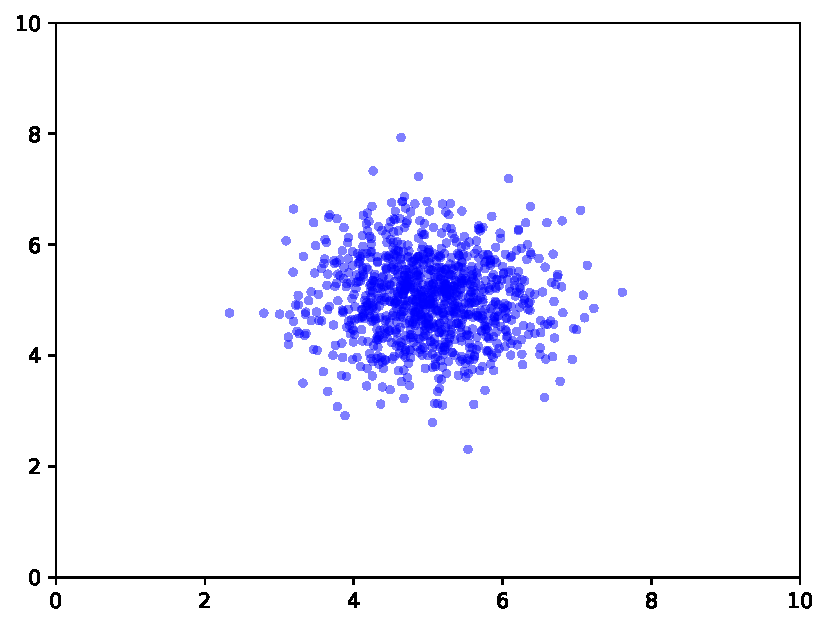
\includegraphics[width=0.19\linewidth]{figures/old/exp_multi_observation_base_N_3_gt_samples}
  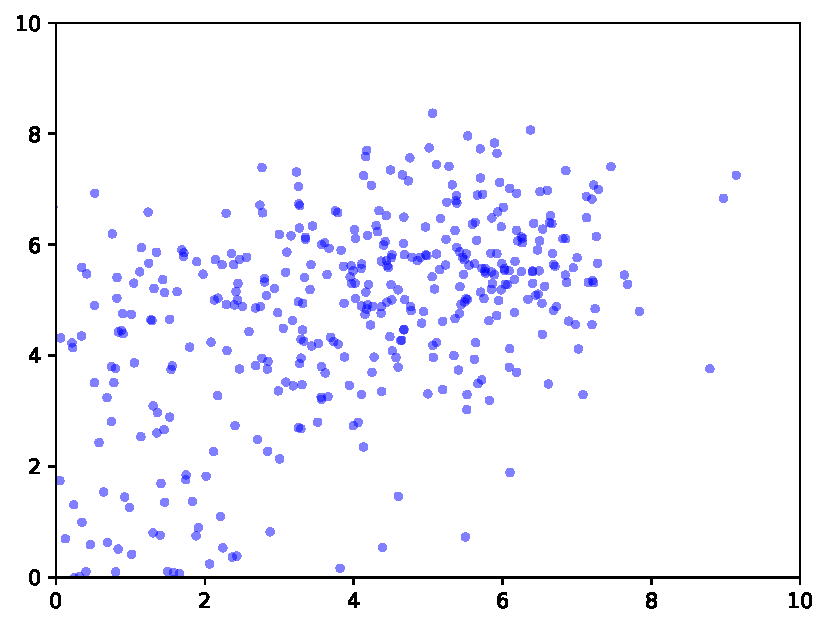
\includegraphics[width=0.19\linewidth]{figures/old/exp_multi_observation_base_N_3_npe_samples}
  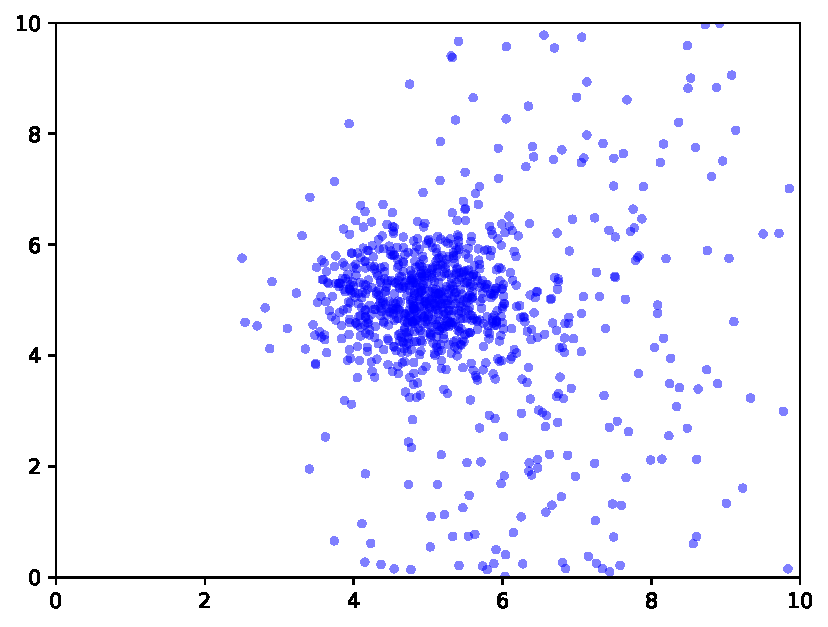
\includegraphics[width=0.19\linewidth]{figures/old/exp_multi_observation_base_N_3_nle_samples}
  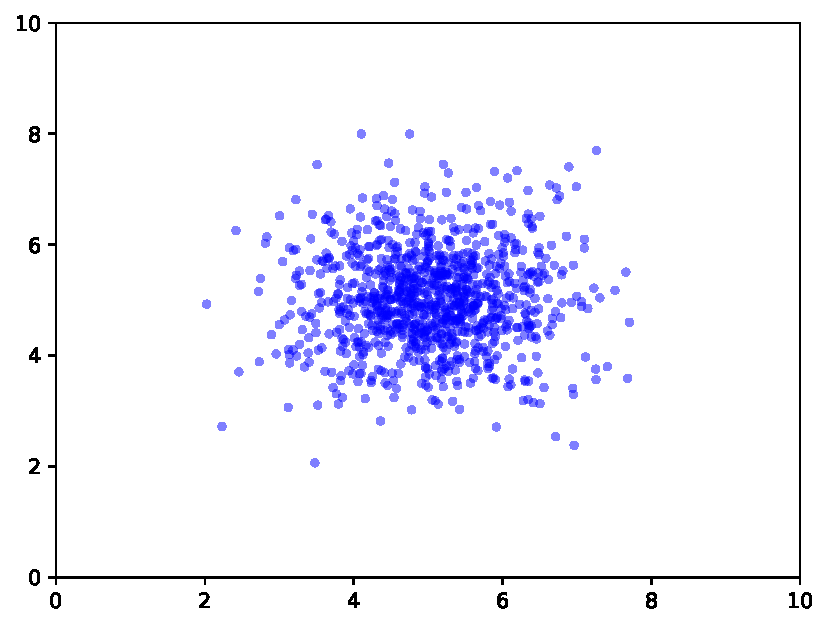
\includegraphics[width=0.19\linewidth]{figures/old/exp_multi_observation_base_N_3_romc_samples}
  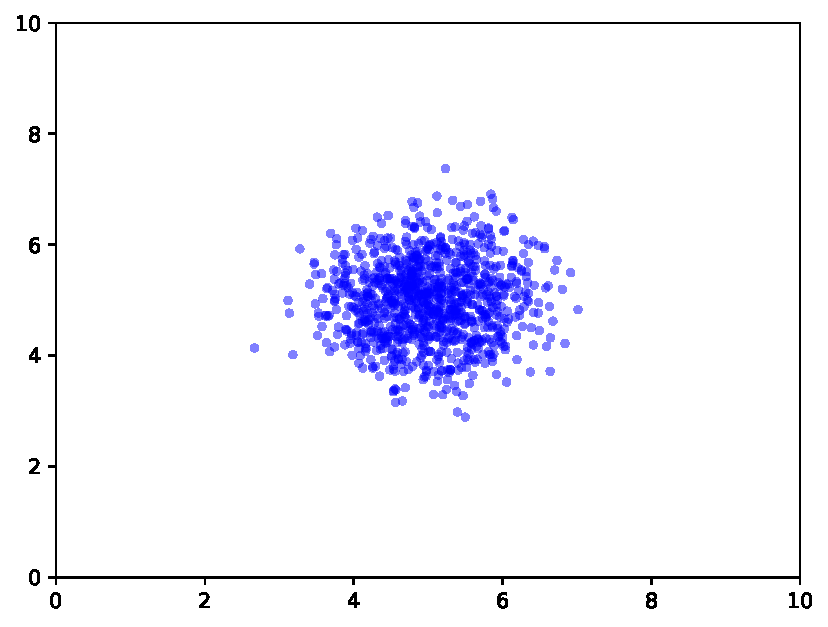
\includegraphics[width=0.19\linewidth]{figures/old/exp_multi_observation_base_N_3_r2omc_samples}\\
  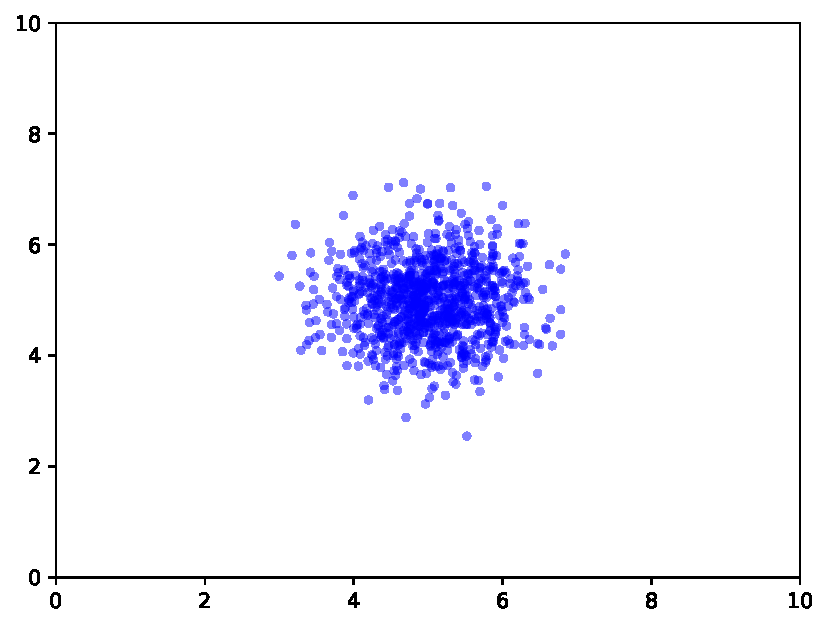
\includegraphics[width=0.19\linewidth]{figures/old/exp_multi_observation_base_N_5_gt_samples}
  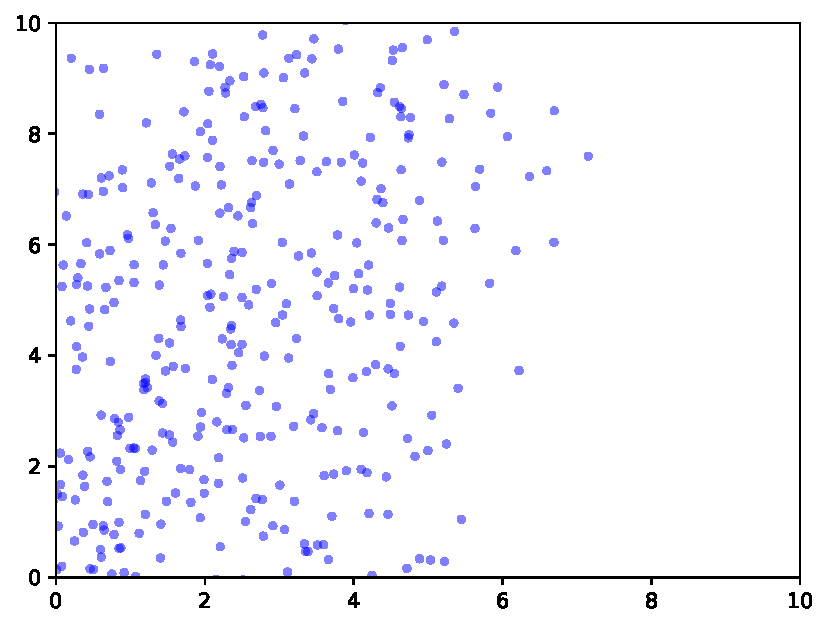
\includegraphics[width=0.19\linewidth]{figures/old/exp_multi_observation_base_N_5_npe_samples}
  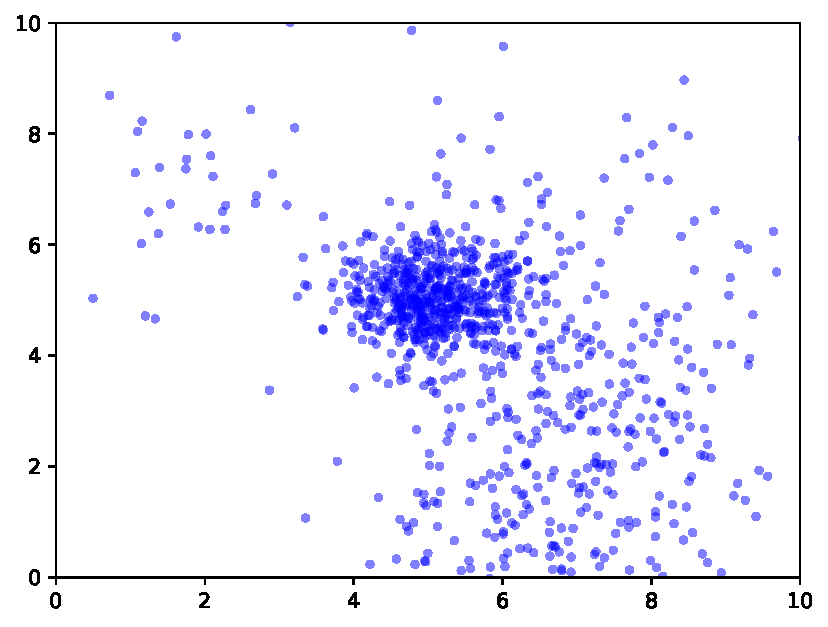
\includegraphics[width=0.19\linewidth]{figures/old/exp_multi_observation_base_N_5_nle_samples}
  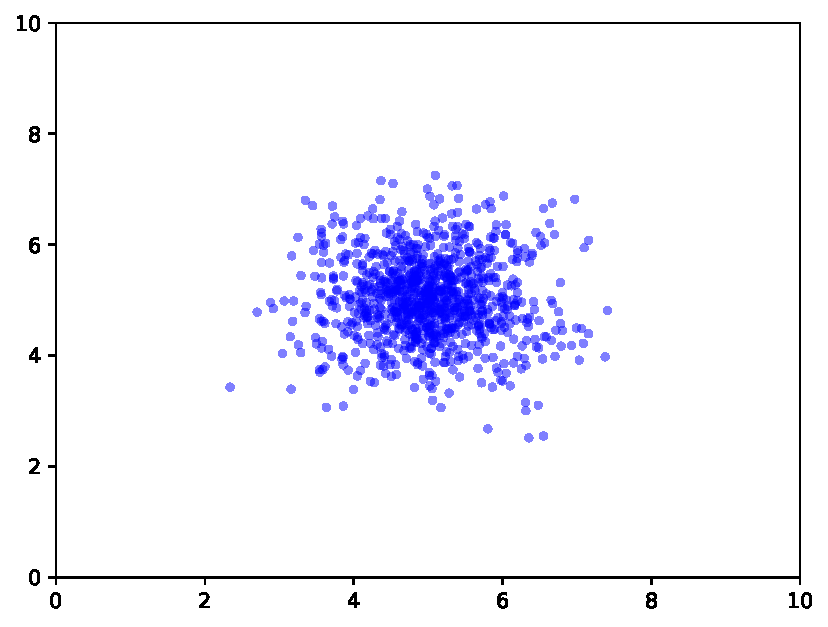
\includegraphics[width=0.19\linewidth]{figures/old/exp_multi_observation_base_N_5_romc_samples}
  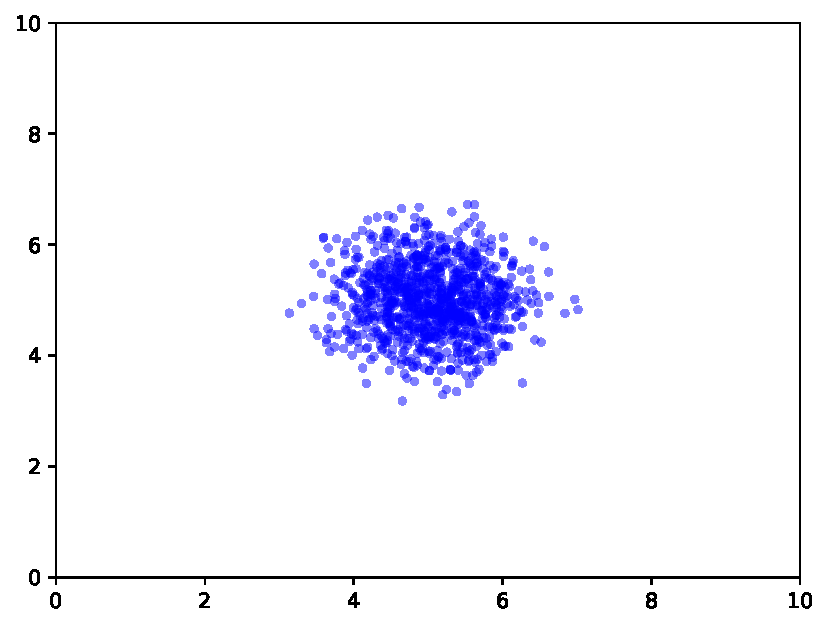
\includegraphics[width=0.19\linewidth]{figures/old/exp_multi_observation_base_N_5_r2omc_samples}\\
  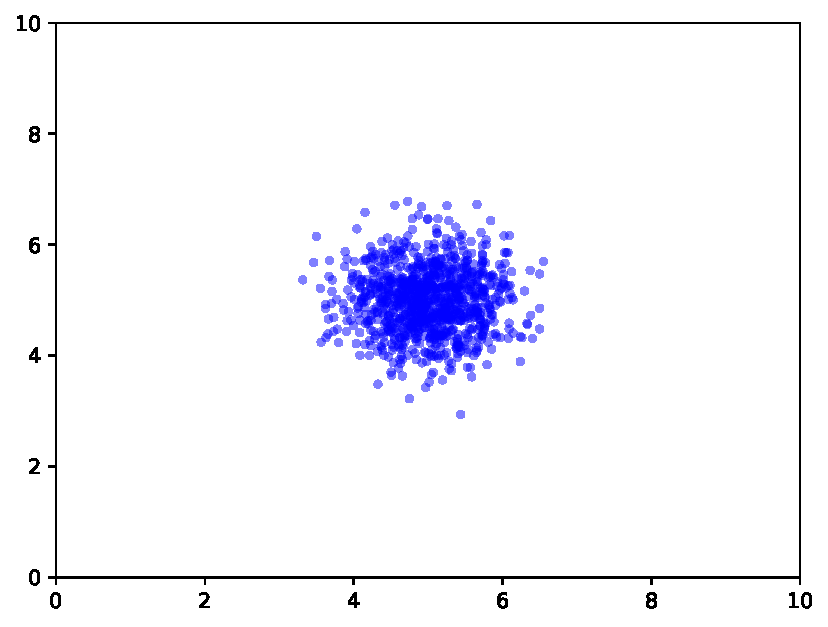
\includegraphics[width=0.19\linewidth]{figures/old/exp_multi_observation_base_N_10_gt_samples}
  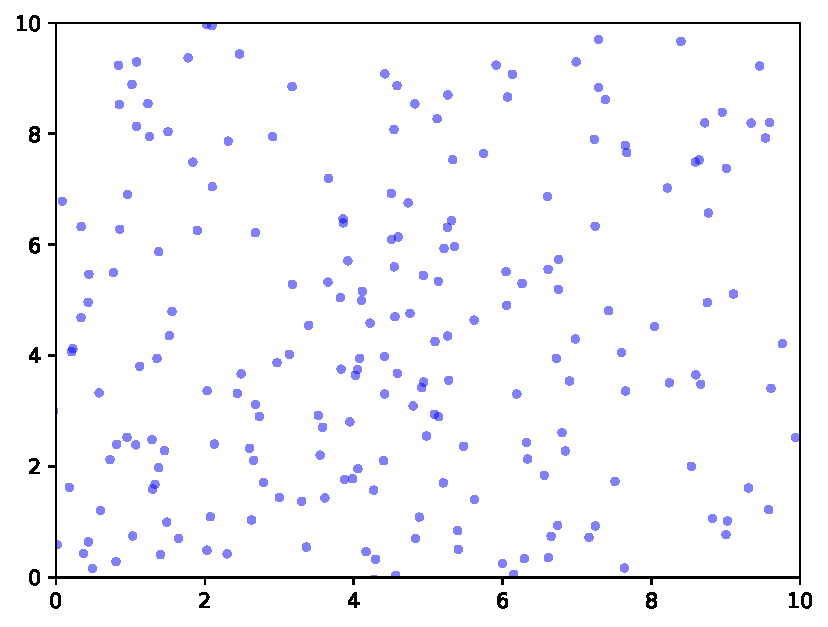
\includegraphics[width=0.19\linewidth]{figures/old/exp_multi_observation_base_N_10_npe_samples}
  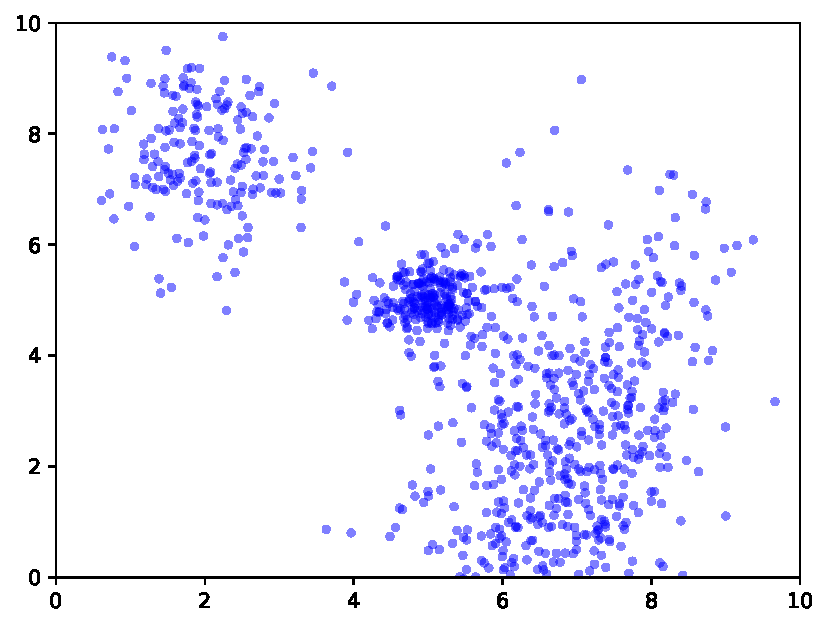
\includegraphics[width=0.19\linewidth]{figures/old/exp_multi_observation_base_N_10_nle_samples}
  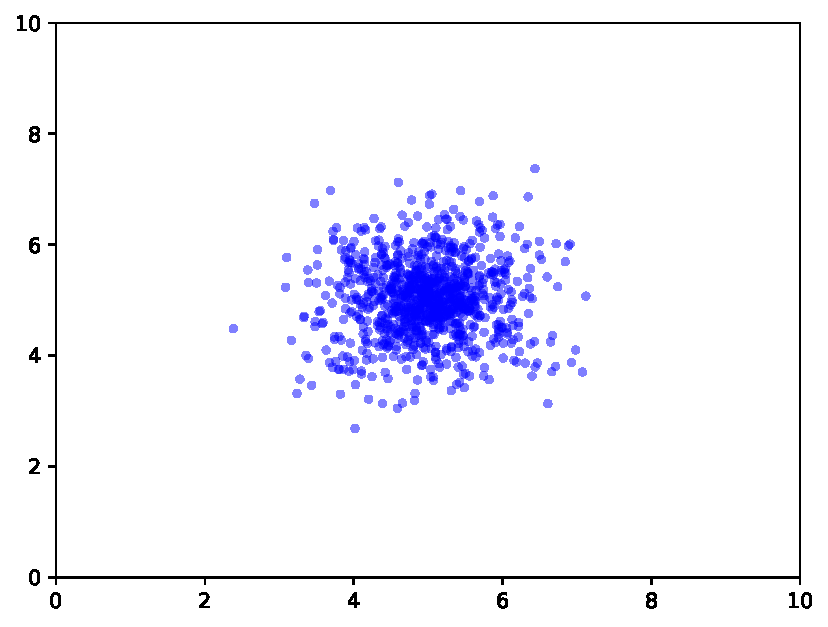
\includegraphics[width=0.19\linewidth]{figures/old/exp_multi_observation_base_N_10_romc_samples}
  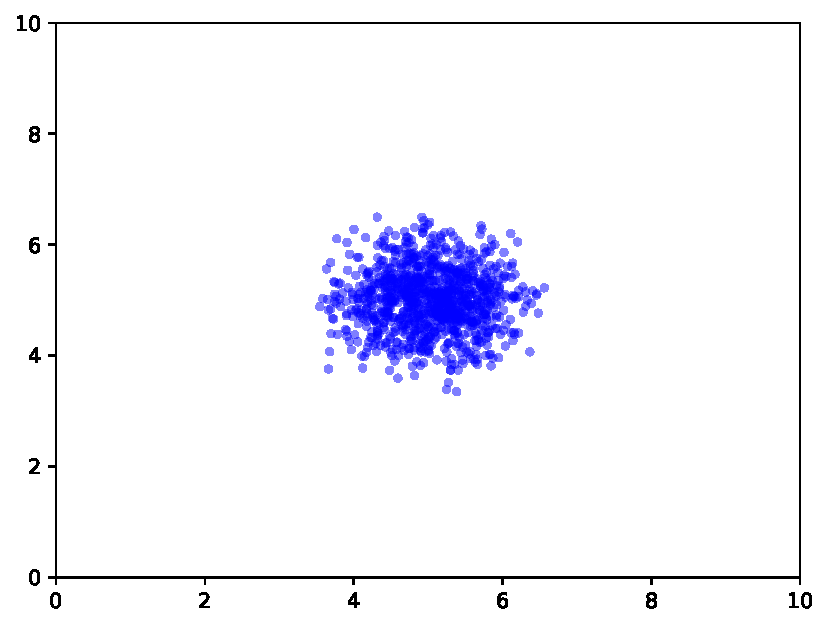
\includegraphics[width=0.19\linewidth]{figures/old/exp_multi_observation_base_N_10_r2omc_samples}\\
  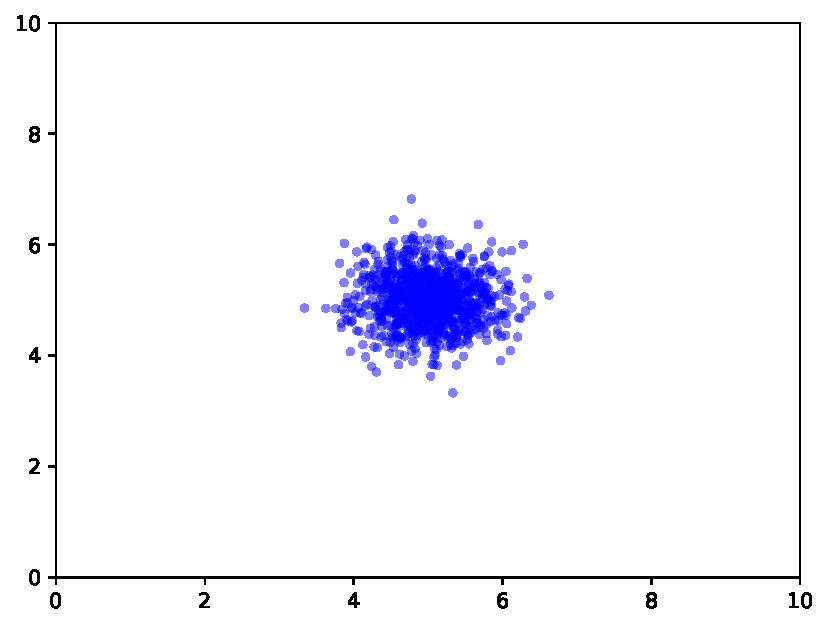
\includegraphics[width=0.19\linewidth]{figures/old/exp_multi_observation_base_N_20_gt_samples}
  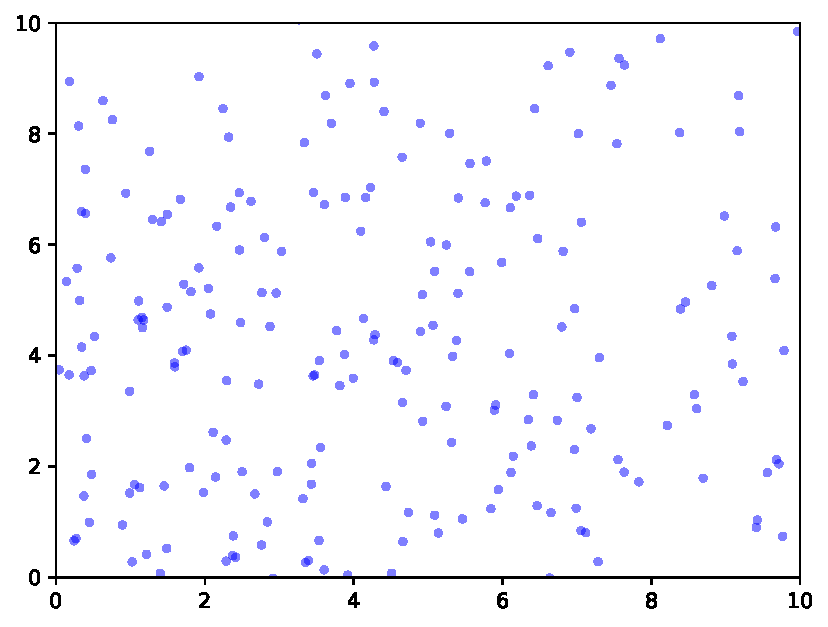
\includegraphics[width=0.19\linewidth]{figures/old/exp_multi_observation_base_N_20_npe_samples}
  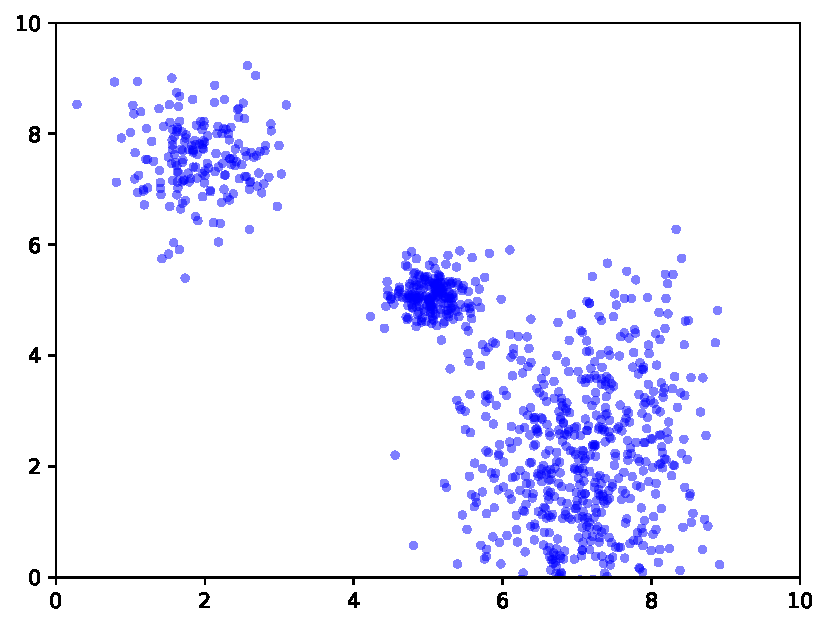
\includegraphics[width=0.19\linewidth]{figures/old/exp_multi_observation_base_N_20_nle_samples}
  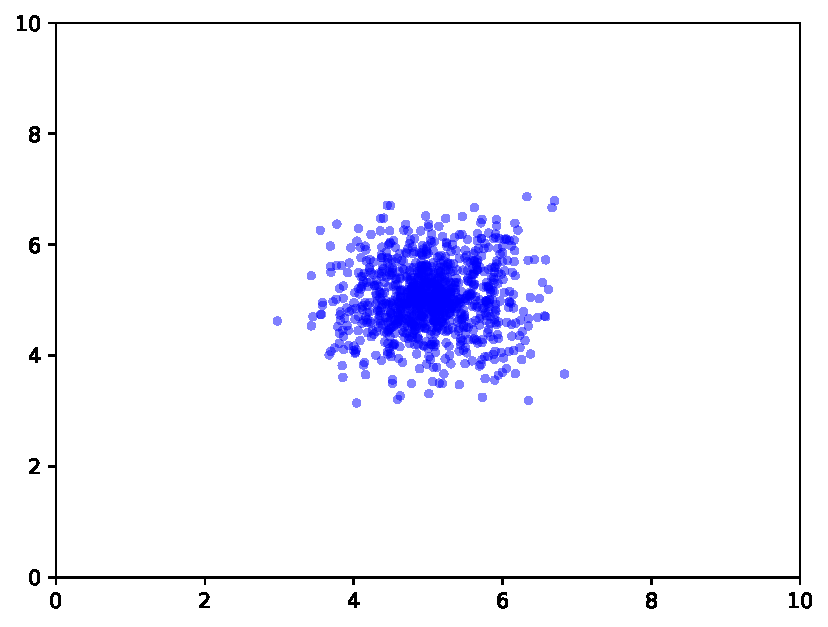
\includegraphics[width=0.19\linewidth]{figures/old/exp_multi_observation_base_N_20_romc_samples}
  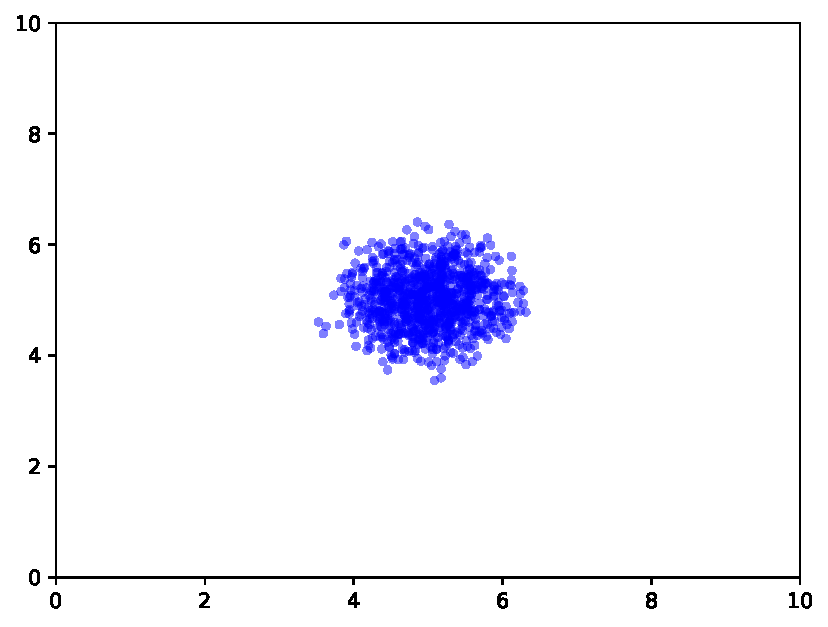
\includegraphics[width=0.19\linewidth]{figures/old/exp_multi_observation_base_N_20_r2omc_samples}
  \caption{Multi observations Base: Left to right: ground truth, NPE, NLE, Naive-ROMC, R2OMC. Top to bottom: $N=3$, $N=5$, $N=10$, $N=10$}
  \label{fig:mo_multi_obs_base}
\end{figure}


\subsubsection{MoG simulator}

\begin{tabular}{@{}ll@{}}
  \textbf{Prior} & $\thb \sim \mathcal{U}(-\mathbf{15}, \mathbf{15})$ \\ [5pt]
  \textbf{Simulator} & $\yb \sim \frac{1}{2} \left( \mathcal{N}(\thb, \sigma_1^2 \mathbf{I}) + \mathcal{N}(-\thb, \sigma_2^2 \mathbf{I}) \right)$, with $\sigma_1=\sigma_2=1$ \\ [5pt]
  \textbf{Dimensionality} & $\thb \in \mathbb{R}^{D}$, $\yb \in \mathbb{R}^{D}$ \\ [5pt]
  \textbf{Observations} & $\{\data_n\}_n^N$ where: \\ [5pt]
  & $\data_n = (5, \ldots, 5) + \epsilon$ for $n \in \{1, \ldots, \frac{N}{2}\}$, \\ [5pt] 
  & $\data_n = (-5, \ldots, -5) + \epsilon$ for $n \in \{\frac{N}{2}+1, \ldots, N\}$ \\ [5pt]
  \textbf{Posterior} & $ p(\thb | \data) \propto
                                    \begin{cases}
                                      \mathcal{N}(\thb; \mathbf{5}, \frac{1}{N} \mathbf{I}) + \mathcal{N}(\thb; -\mathbf{5}, \frac{1}{N} \mathbf{I}), & \text{if } \thb \in [-15, 15]^D, \\
                                      0, & \text{otherwise}.
                                    \end{cases} $ \\ [5pt]
\end{tabular}

\textbf{Proof of the posterior:}
\begin{equation}
  p(\thb|\{\data_n\}) \appropto 
  \begin{cases}
    \mathcal{N}(\thb; \mathbf{5}, \frac{1}{N} \mathbf{I}) + \mathcal{N}(\thb; -\mathbf{5}, \frac{1}{N}\mathbf{I}), & \text{if } \thb \in [-15, 15]^D, \\
    0, & \text{otherwise}.
  \end{cases}
  \label{eq:mog_mog_mult_obs}
\end{equation}
The proof is similar to the one in Eq.~(\ref{eq:intro-multiple}).

In Figure~\ref{fig:mog_multi_obs}, we present the results for the MoG simulator with multiple observations.


\begin{figure}[]
  \centering
  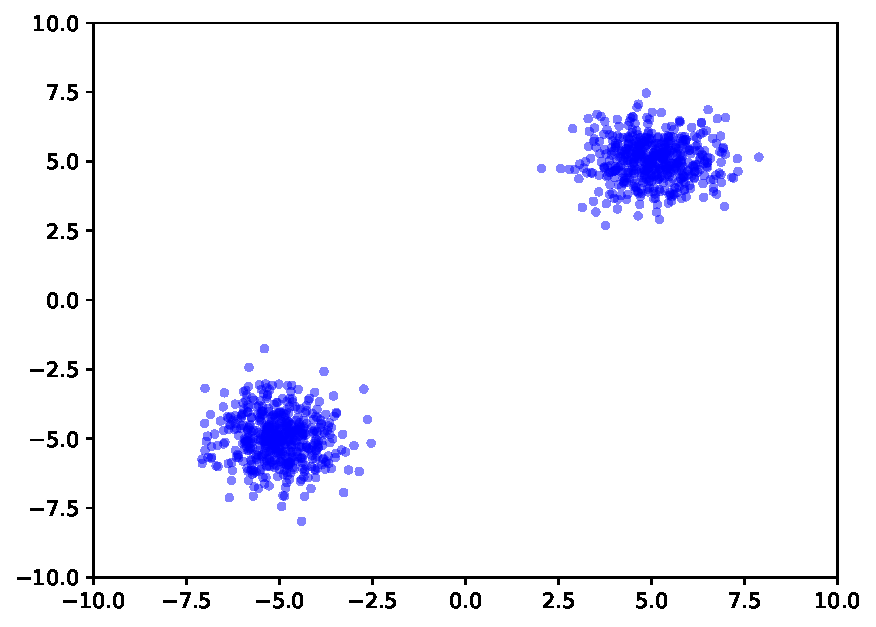
\includegraphics[width=0.19\linewidth]{figures/old/exp_multi_observation_MoG_N_2_gt_samples}
  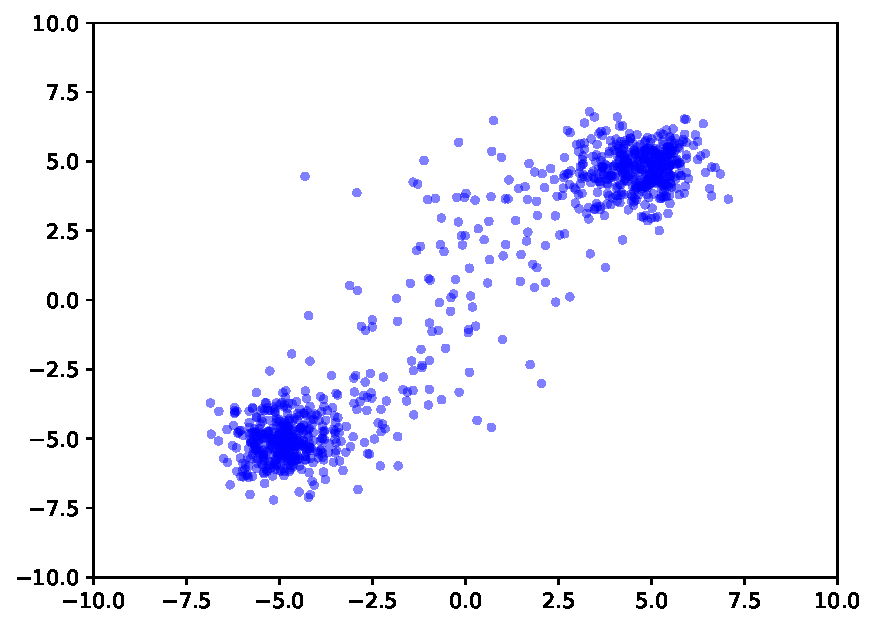
\includegraphics[width=0.19\linewidth]{figures/old/exp_multi_observation_MoG_N_2_npe_samples}
  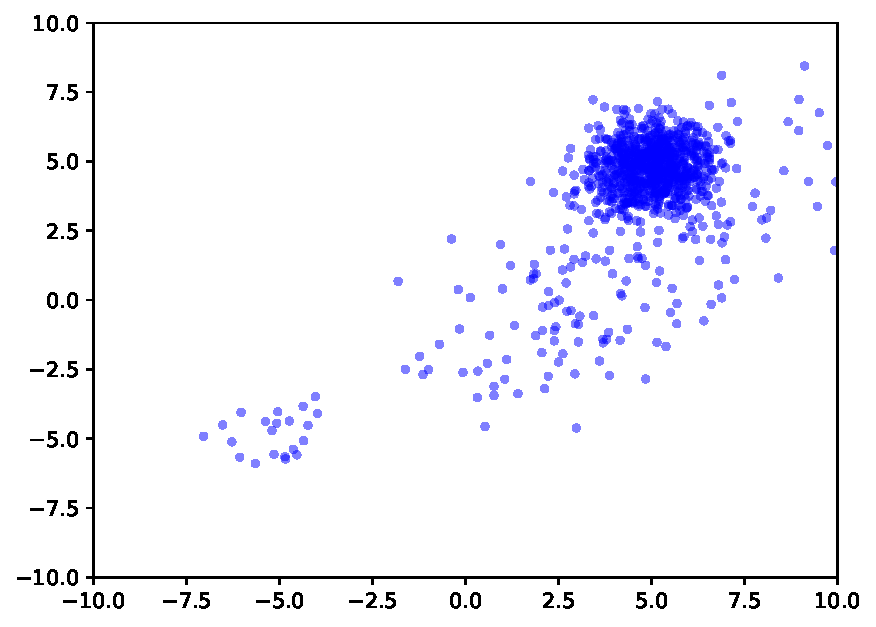
\includegraphics[width=0.19\linewidth]{figures/old/exp_multi_observation_MoG_N_2_nle_samples}
  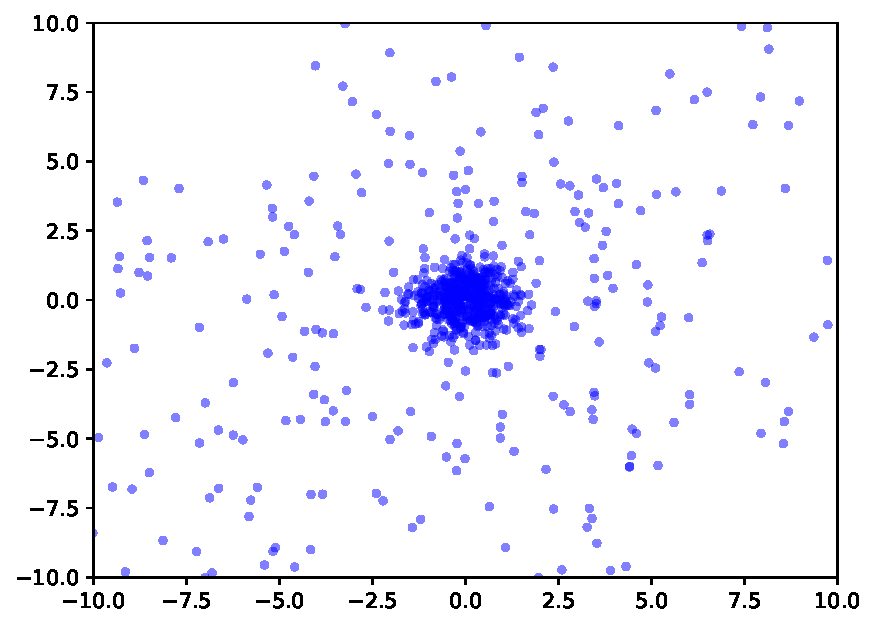
\includegraphics[width=0.19\linewidth]{figures/old/exp_multi_observation_MoG_N_2_romc_samples}
  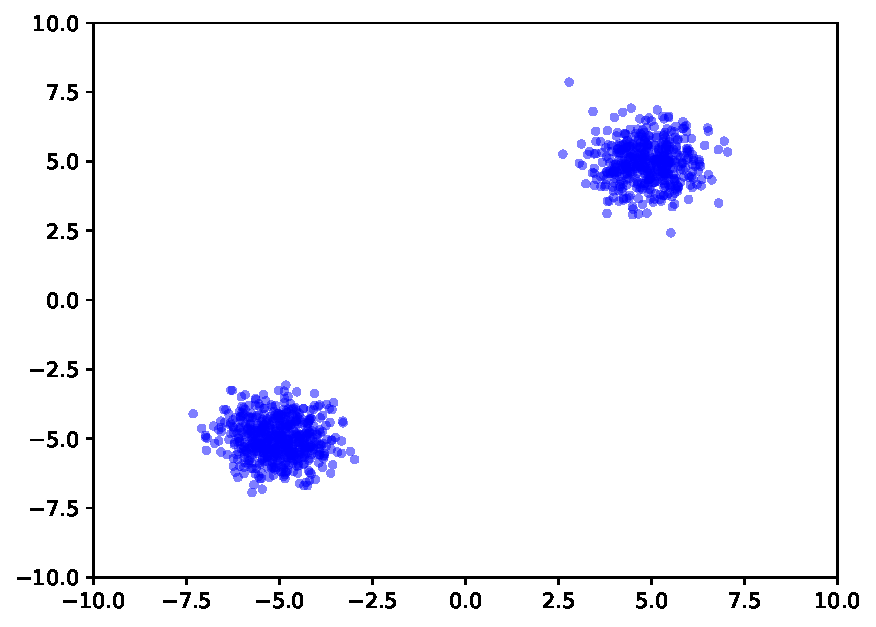
\includegraphics[width=0.19\linewidth]{figures/old/exp_multi_observation_MoG_N_2_r2omc_samples}\\
  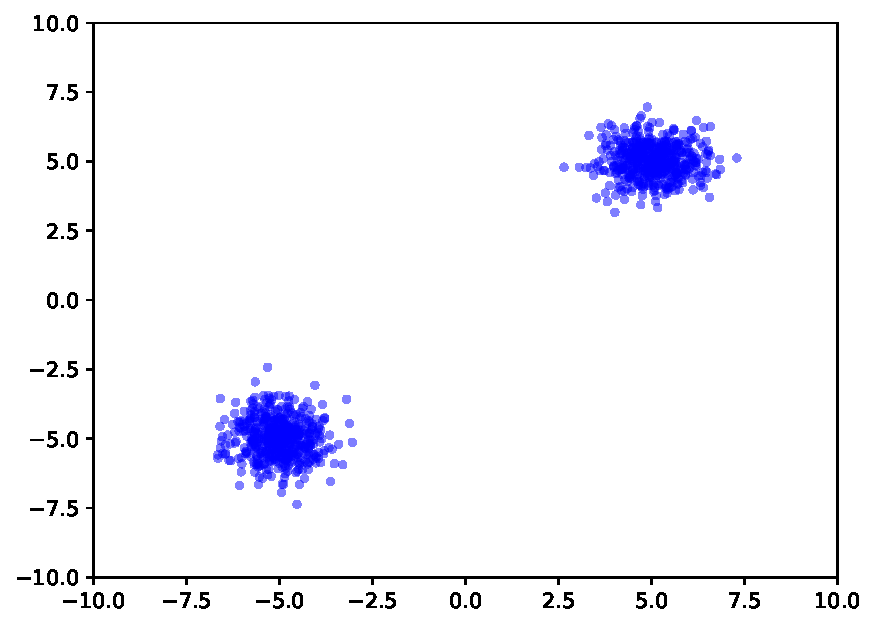
\includegraphics[width=0.19\linewidth]{figures/old/exp_multi_observation_MoG_N_5_gt_samples}
  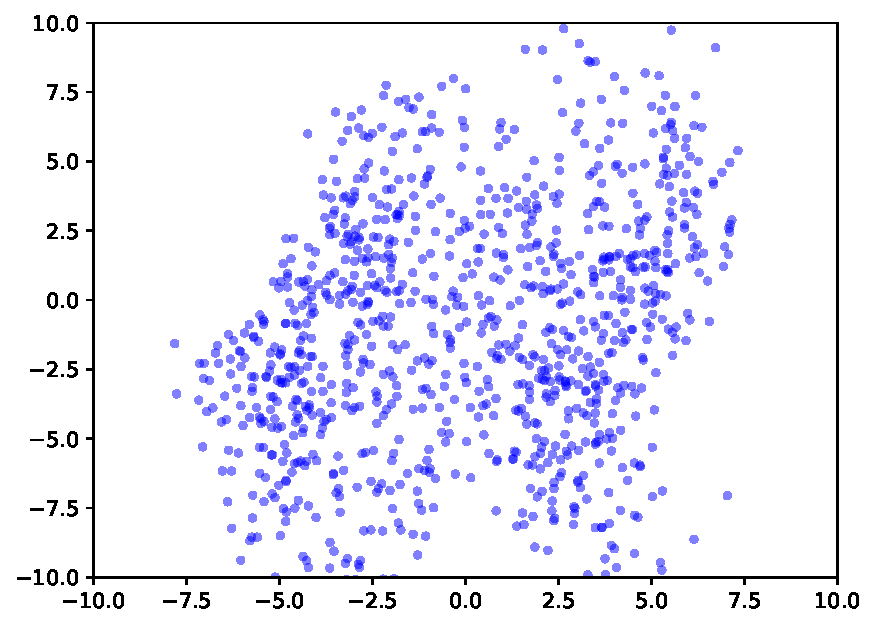
\includegraphics[width=0.19\linewidth]{figures/old/exp_multi_observation_MoG_N_5_npe_samples}
  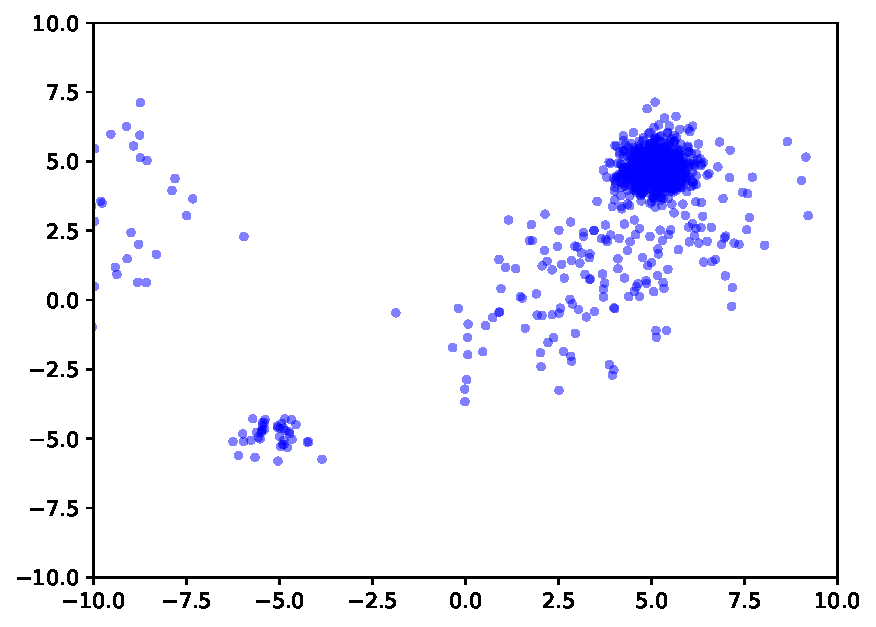
\includegraphics[width=0.19\linewidth]{figures/old/exp_multi_observation_MoG_N_5_nle_samples}
  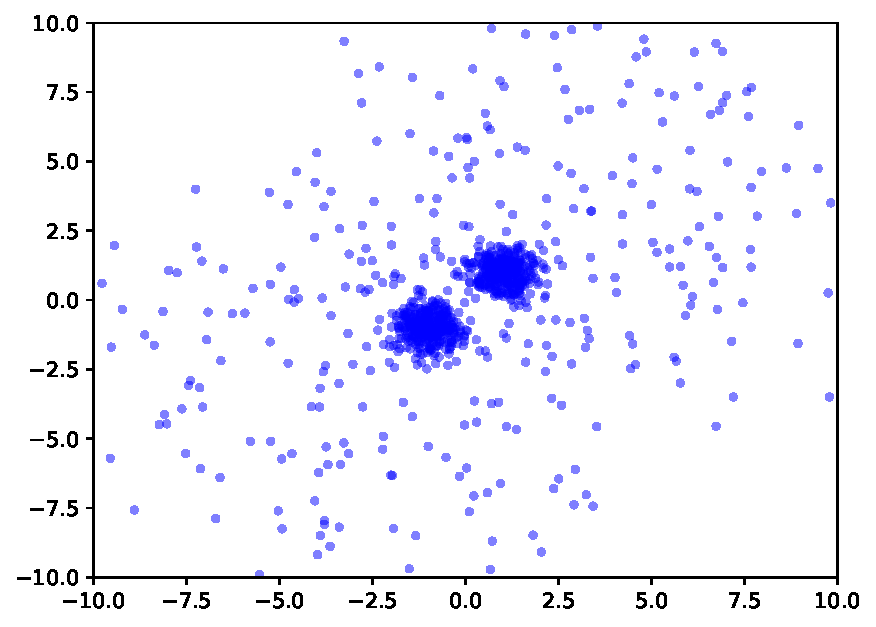
\includegraphics[width=0.19\linewidth]{figures/old/exp_multi_observation_MoG_N_5_romc_samples}
  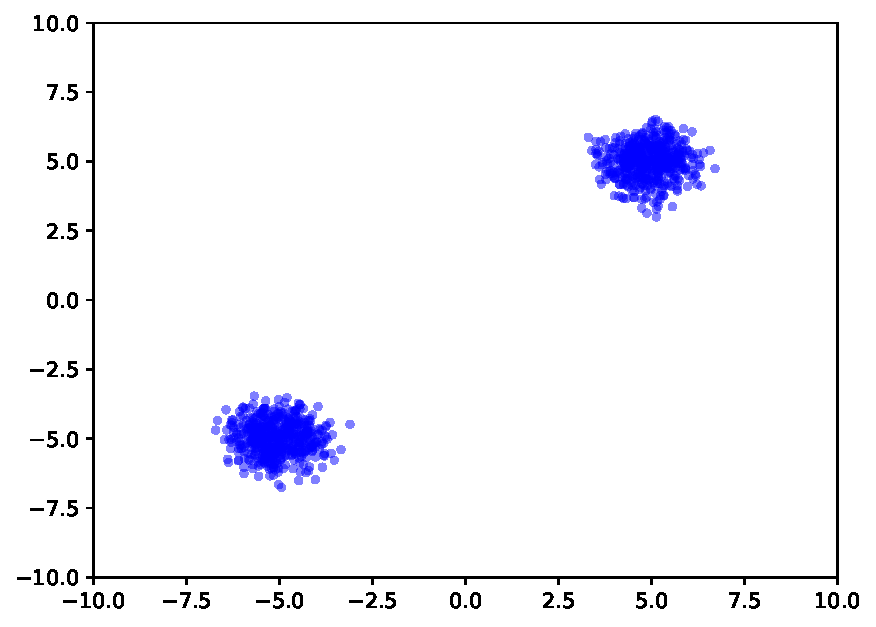
\includegraphics[width=0.19\linewidth]{figures/old/exp_multi_observation_MoG_N_5_r2omc_samples}\\
  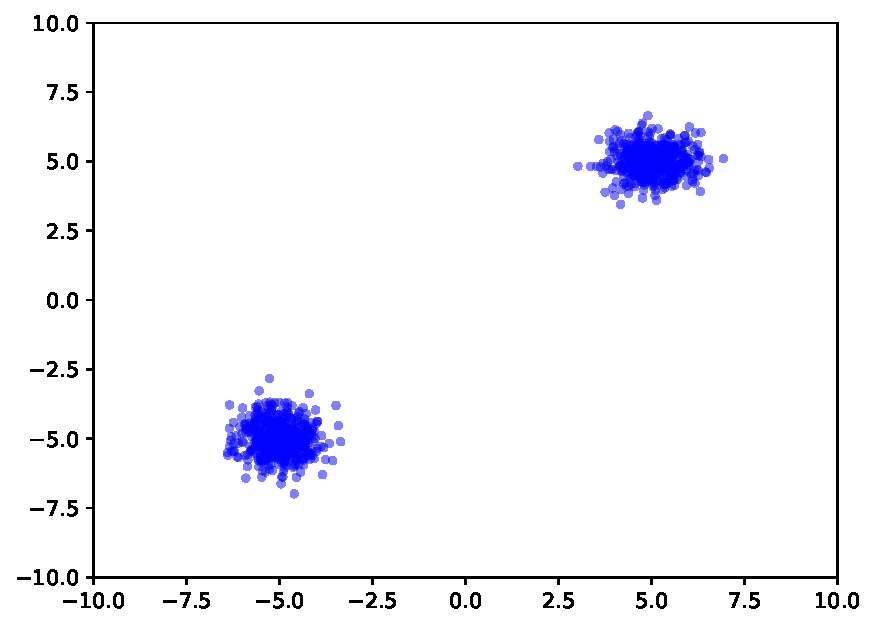
\includegraphics[width=0.19\linewidth]{figures/old/exp_multi_observation_MoG_N_10_gt_samples}
  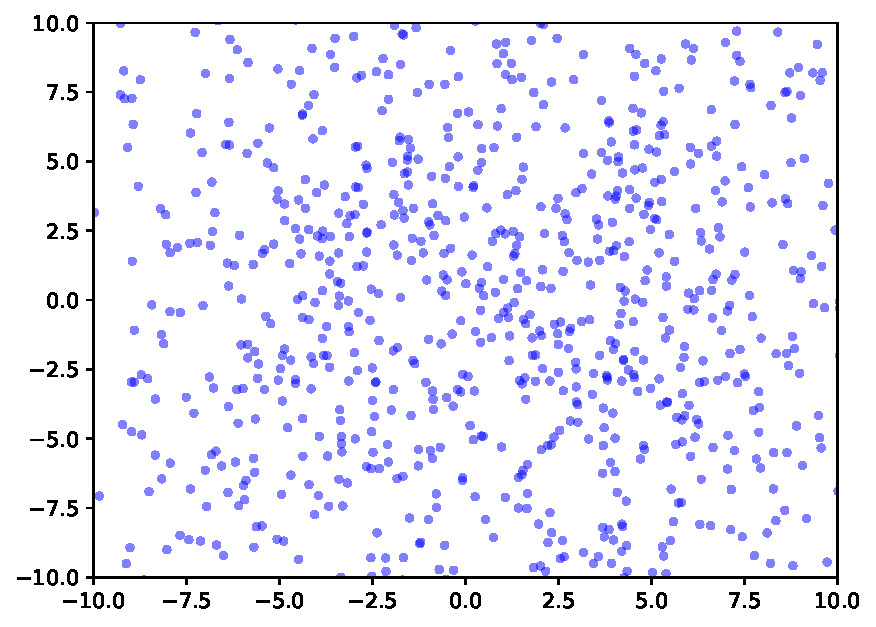
\includegraphics[width=0.19\linewidth]{figures/old/exp_multi_observation_MoG_N_10_npe_samples}
  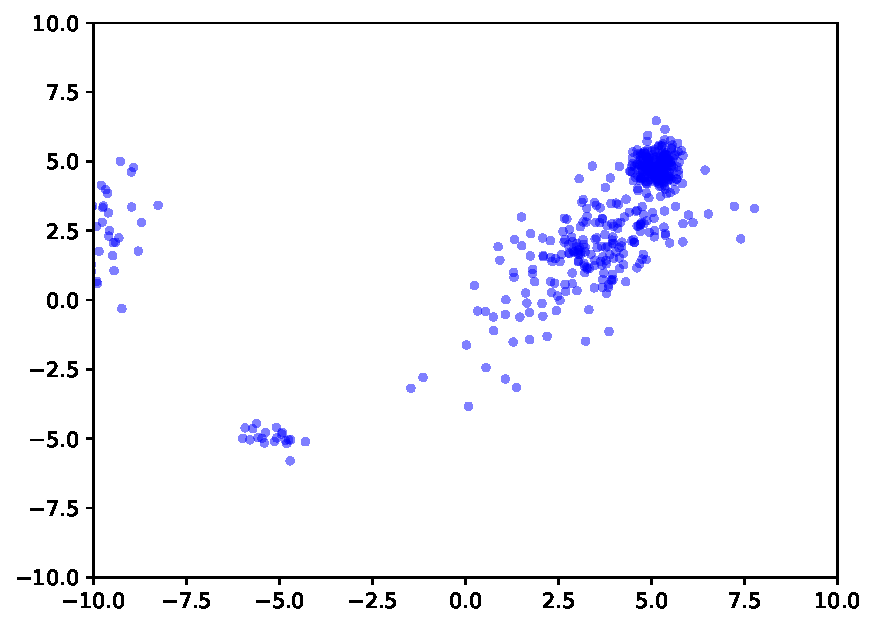
\includegraphics[width=0.19\linewidth]{figures/old/exp_multi_observation_MoG_N_10_nle_samples}
  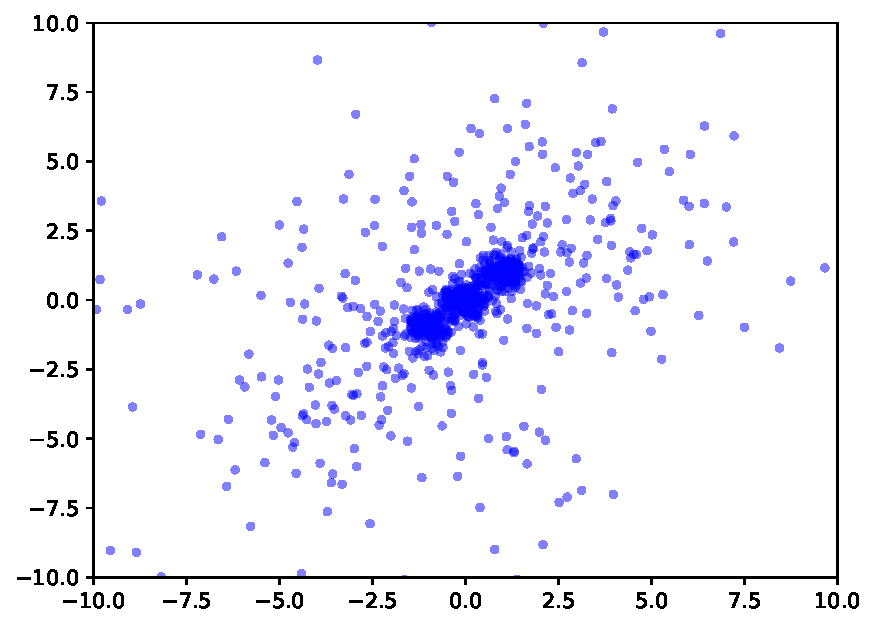
\includegraphics[width=0.19\linewidth]{figures/old/exp_multi_observation_MoG_N_10_romc_samples}
  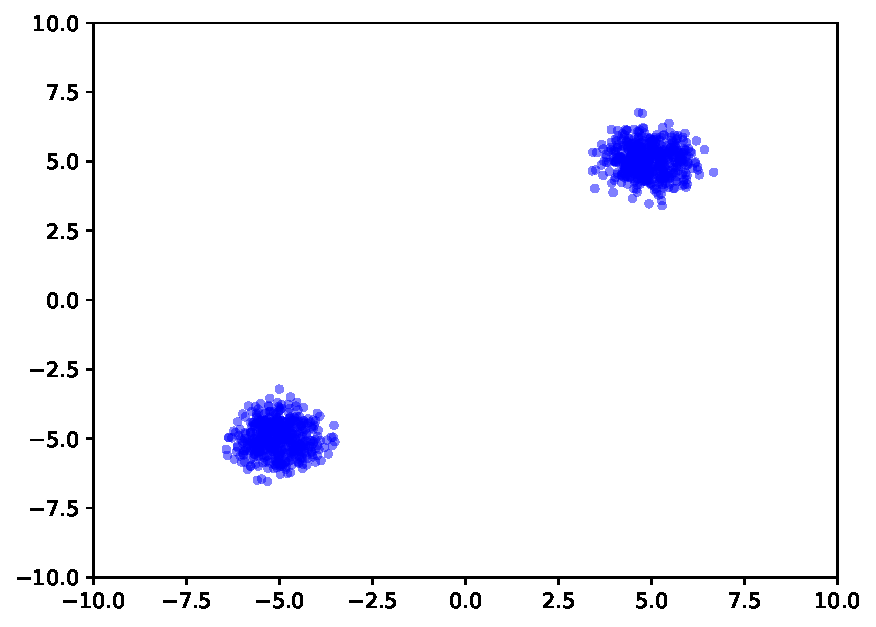
\includegraphics[width=0.19\linewidth]{figures/old/exp_multi_observation_MoG_N_10_r2omc_samples}\\
  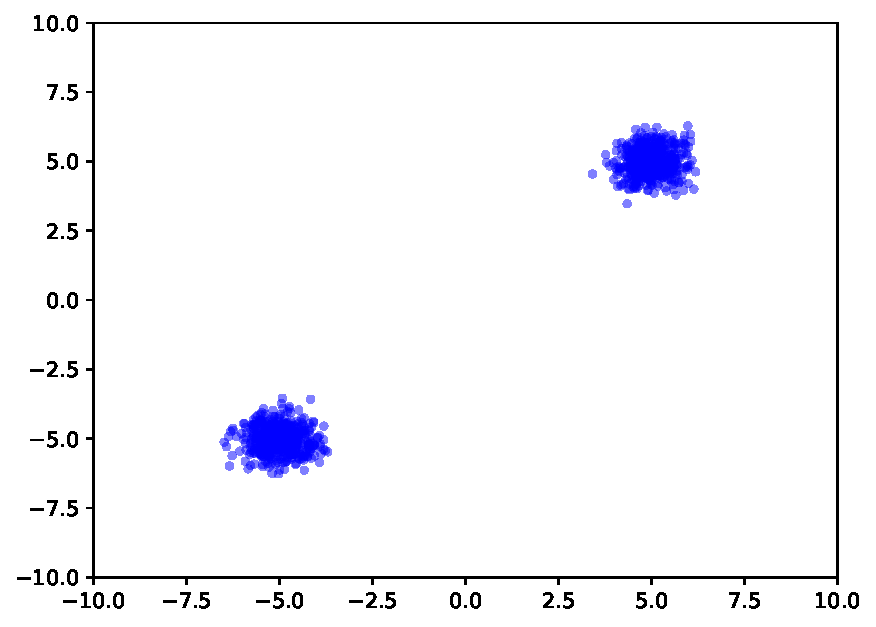
\includegraphics[width=0.19\linewidth]{figures/old/exp_multi_observation_MoG_N_20_gt_samples}
  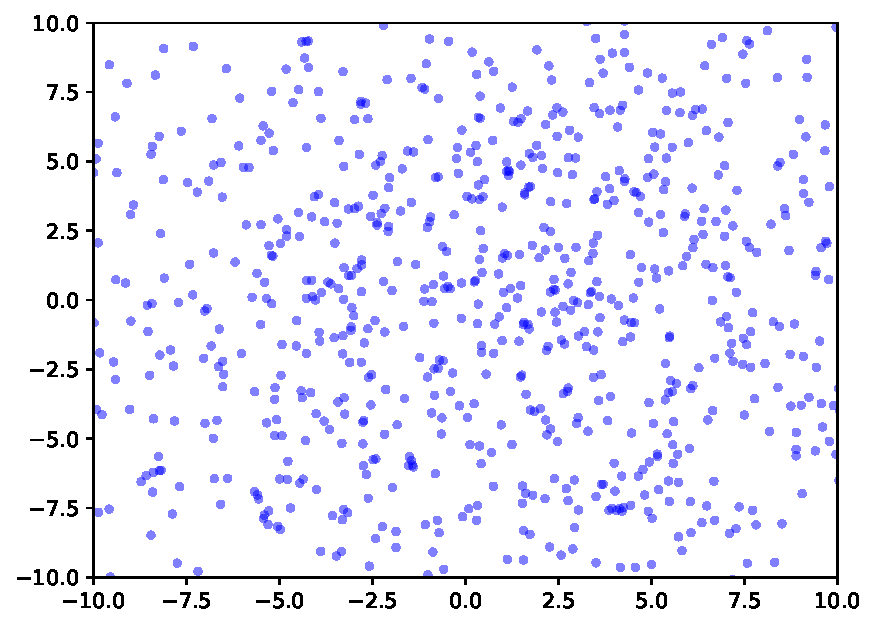
\includegraphics[width=0.19\linewidth]{figures/old/exp_multi_observation_MoG_N_20_npe_samples}
  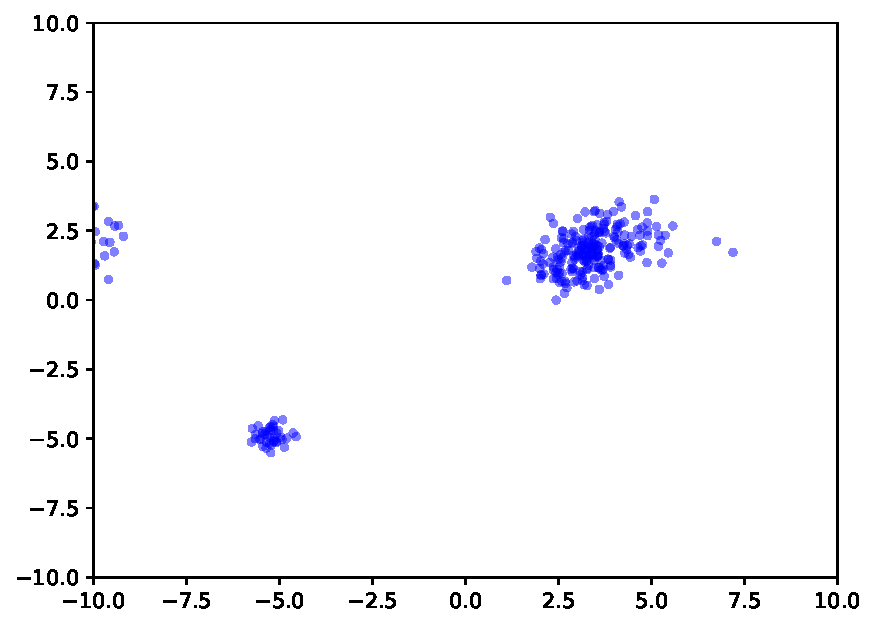
\includegraphics[width=0.19\linewidth]{figures/old/exp_multi_observation_MoG_N_20_nle_samples}
  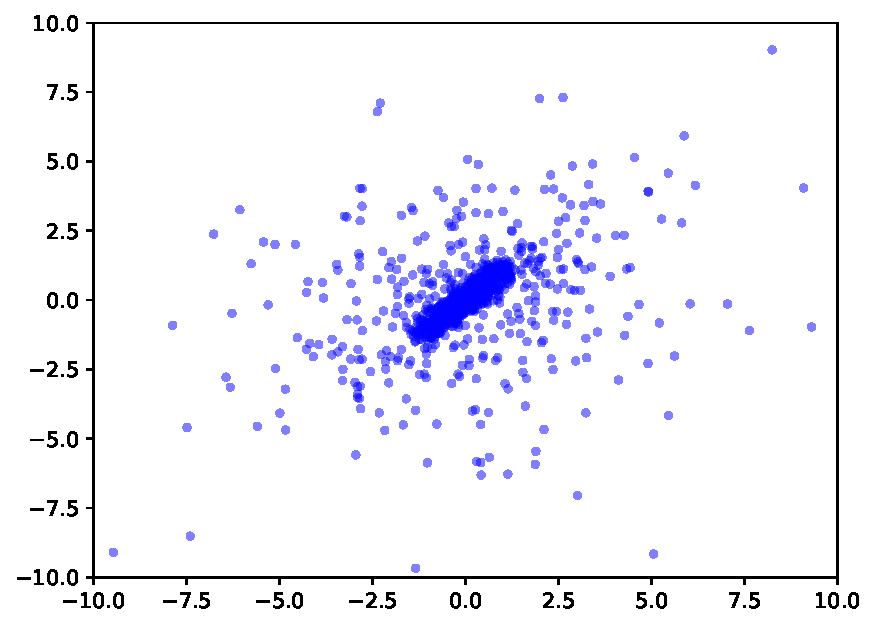
\includegraphics[width=0.19\linewidth]{figures/old/exp_multi_observation_MoG_N_20_romc_samples}
  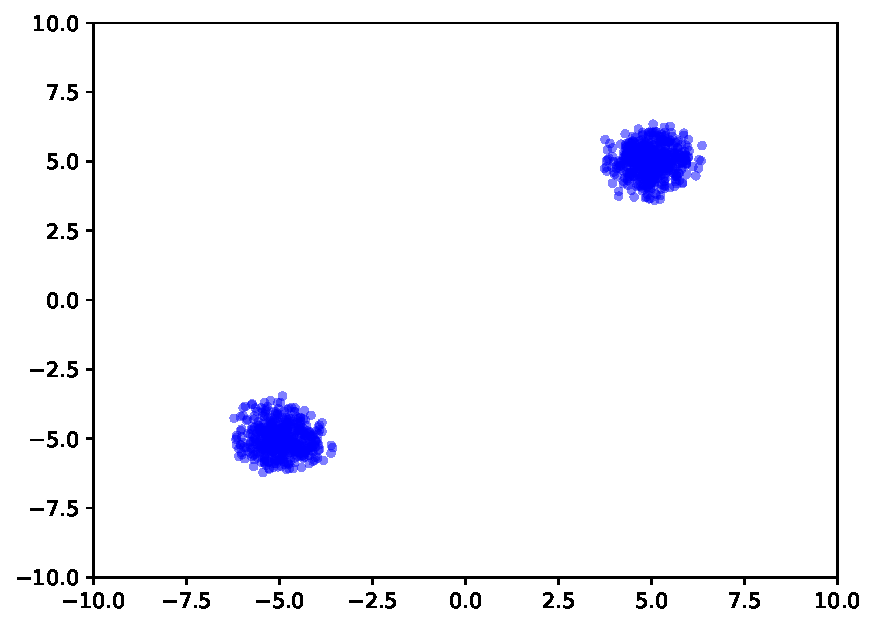
\includegraphics[width=0.19\linewidth]{figures/old/exp_multi_observation_MoG_N_20_r2omc_samples}
  \caption{Multi observations MoG: Left to right: ground truth, NPE, NLE, Naive-ROMC, R2OMC. Top to bottom: $N=3$, $N=5$, $N=10$, $N=10$}
  \label{fig:mog_multi_obs}
\end{figure}

\subsection{SBI - Mixtures of Gaussians (T.7)}

We here provide additional information on example T.7 of the SBI benchmark~\cite{lueckmann2021benchmarking}.
It tests inference of the mean of a mixture of two $2$-D Gaussians, one with much broader covariance than the other

\begin{tabular}{@{}ll@{}}
  \textbf{Prior} & $\thb \sim \mathcal{U}(-\mathbf{10}, \mathbf{10})$ \\ [5pt]
  \textbf{Simulator} & $\yb \sim 0.5 (\mathcal{N}(\thb, \mathbf{I}) + \mathcal{N}(\thb, \sigma^2 \mathbf{I}))$, with $\sigma^2 = 0.01$ \\ [5pt]
  \textbf{Dimensionality} & $\thb \in \mathbb{R}^{2}$, $\yb \in \mathbb{R}^{2}$ \\ [5pt]
\end{tabular}

\paragraph{Results.}

We evaluate \rromc~using a simulation budget of $S=1000$ and $S=10000$ seeds.
The \texttt{C2ST} score is computed by comparing 1000 samples from the true posterior (we randomly select 1000 from the 10000 that are provided by the SBI benchmark)
with 1000 samples generated from the \rromc~approximate posterior.
The results are illustrated in Figure~\ref{fig:exp_sbi_gaussian_mixture}.

\begin{figure}[ht]
  \centering
  \begin{subfigure}[b]{0.32\linewidth}
    \centering
    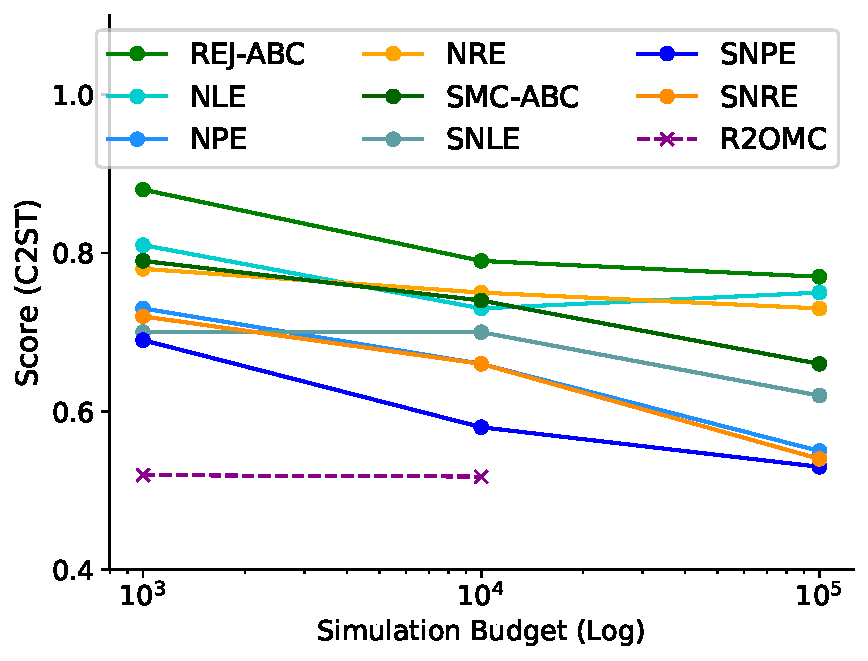
\includegraphics[width=\linewidth]{figures/old/gaussian_mixture}
    \caption{\texttt{C2ST} score}
  \end{subfigure}
  \hfill
  \begin{subfigure}[b]{0.32\linewidth}
    \centering
    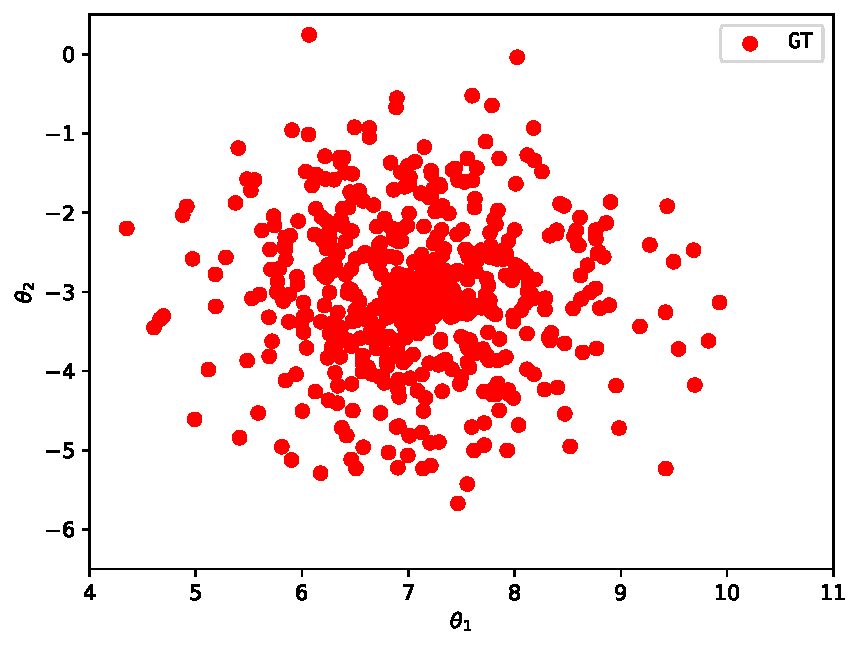
\includegraphics[width=\linewidth]{figures/old/exp_sbi_gaussian_mixture_gt}
    \caption{Ground truth samples}
  \end{subfigure}
  \hfill
  \begin{subfigure}[b]{0.32\linewidth}
    \centering
    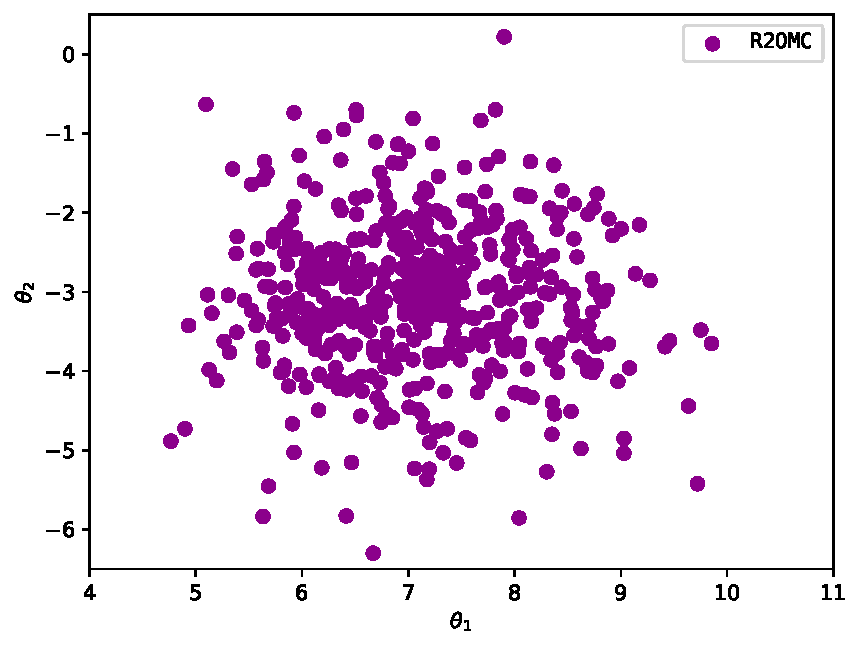
\includegraphics[width=\linewidth]{figures/old/exp_sbi_gaussian_mixture_r2omc}
    \caption{Samples by R2OMC}
  \end{subfigure}
  \caption{T.7: Gaussian Mixture. From left to right: \texttt{C2ST} score, ground truth samples, and samples by R2OMC.}
  \label{fig:exp_sbi_gaussian_mixture}
\end{figure}

\subsection{SBI - Two Moons (T.8)}

We here provide additional information on example T.8 of the SBI benchmark~\cite{lueckmann2021benchmarking}.
It tests inference when the posterior exhibits both global (bimodality) and local (crescent shape) structure to illustrate how algorithms deal with multimodality:

\begin{tabular}{@{}ll@{}}
  \textbf{Prior} & $\thb \sim \mathcal{U}(-\mathbf{1}, \mathbf{1})$ \\ [5pt]
  \textbf{Simulator} & $\yb \sim \begin{bmatrix} 
    r \cos(\alpha) + 0.25 \\ 
    r \sin(\alpha)
  \end{bmatrix} + \begin{bmatrix} 
    |\theta_1 + \theta_2|/\sqrt{2} \\ 
    (-\theta_1 + \theta_2)/\sqrt{2}
  \end{bmatrix}$, where $r \sim \mathcal{N}(0.1, 0.01^2)$ and $\alpha \sim \mathcal{U}(-\pi/2, \pi/2)$ \\ [10pt]
  \textbf{Dimensionality} & $\thb \in \mathbb{R}^{2}$, $\yb \in \mathbb{R}^{2}$ \\ [5pt]
\end{tabular}

\paragraph{Results.}

We evaluate \rromc~using a simulation budget of $S=1000$ and $S=10000$ seeds.
The \texttt{C2ST} score is computed by comparing 1000 samples from the true posterior (we randomly select 1000 from the 10000 that are provided by the SBI benchmark)
with 1000 samples generated from the \rromc~approximate posterior.
The results are illustrated in Figure~\ref{fig:exp_sbi_gaussian_mixture}.
We observe that \rromc~is able to capture the bimodal structure of the posterior, perfectly replicating the ground truth samples.

\begin{figure}[ht]
  \centering
  \begin{subfigure}[b]{0.32\linewidth}
    \centering
    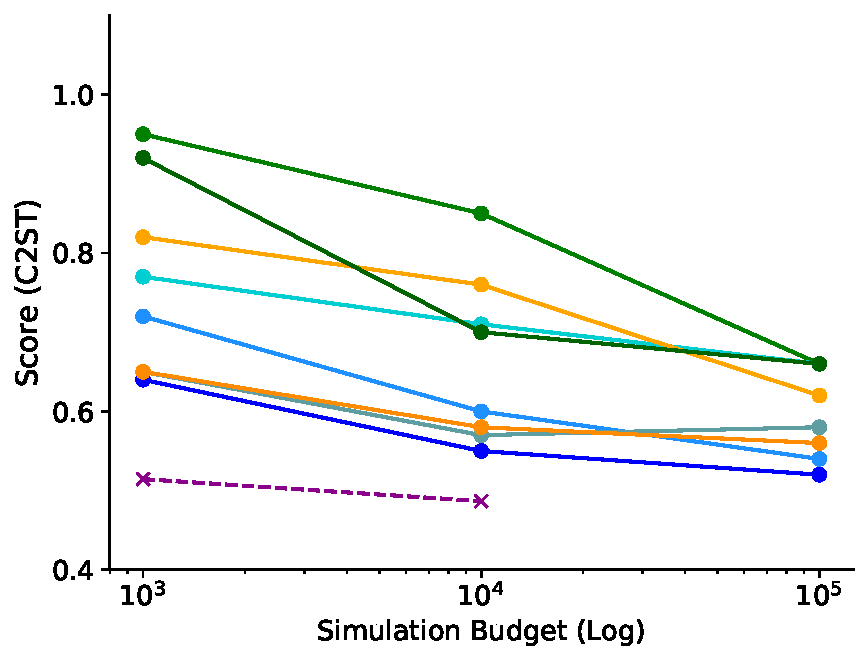
\includegraphics[width=\linewidth]{figures/old/two_moons}
    \caption{\texttt{C2ST} score}
  \end{subfigure}
  \hfill
  \begin{subfigure}[b]{0.32\linewidth}
    \centering
    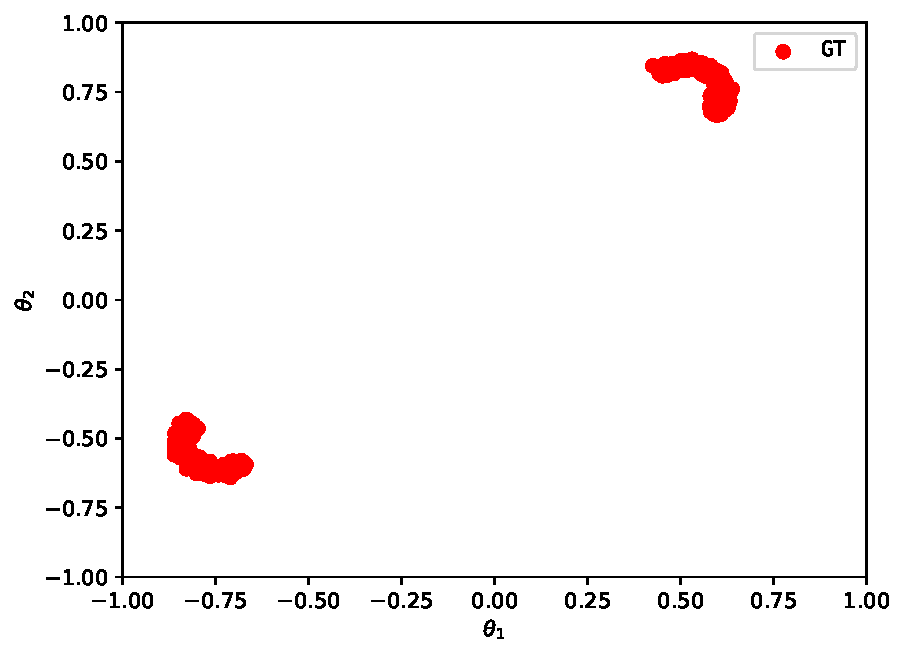
\includegraphics[width=\linewidth]{figures/old/exp_sbi_two_moons_gt}
    \caption{Ground truth samples}
  \end{subfigure}
  \hfill
  \begin{subfigure}[b]{0.32\linewidth}
    \centering
    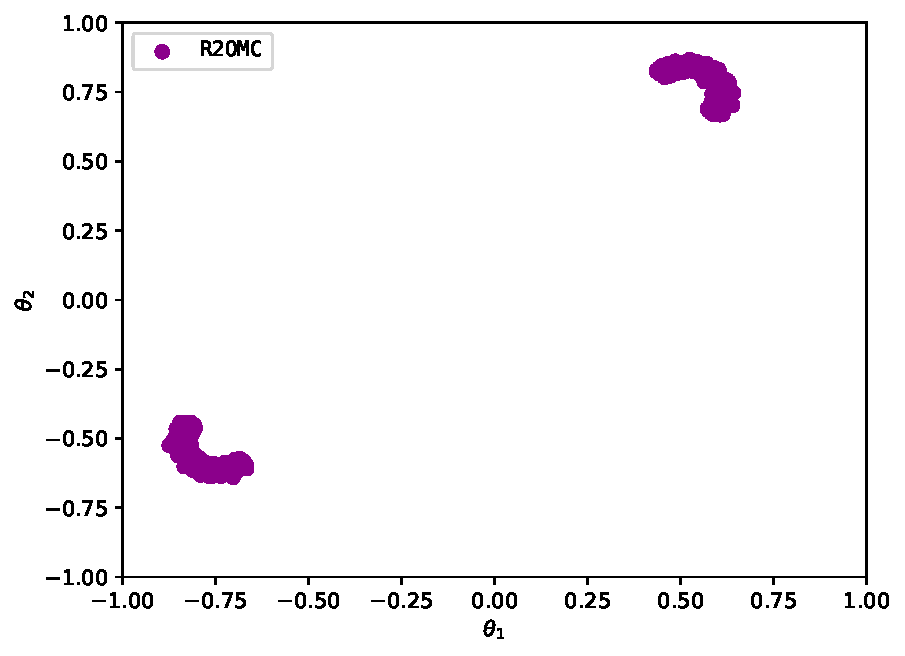
\includegraphics[width=\linewidth]{figures/old/exp_sbi_two_moons_r2omc}
    \caption{Samples by R2OMC}
  \end{subfigure}
  \caption{T.8: Two Moons. From left to right: \texttt{C2ST} score, ground truth samples, and samples by R2OMC.}
  \label{fig:exp_sbi_two_moons}
\end{figure}

\clearpage

\section{Additional results}
\label{sec:additional-experiments}

We here present some additional experiments that were not included in the main text.

% \subsection{SBI - Gaussian Linear Uniform (T.2)}

% This is the T.2 from the SBI benchmark~\cite{lueckmann2021benchmarking}.
% It tests inference of the mean of a $10$-D Gaussian model with fixed covariance.
% The posterior is a truncated Gaussian distribution:

% \begin{tabular}{@{}ll@{}}
%   \textbf{Prior} & $\thb \sim \mathcal{U}(-1, 1)$ \\[5pt]
%   \textbf{Simulator} & $\yb \sim \mathcal{N}(\thb, 0.1 \odot \mathbf{I})$ \\[5pt]
%   \textbf{Dimensionality} & $\thb \in \mathbb{R}^{10}$, $\yb \in \mathbb{R}^{10}$ \\[5pt]
% \end{tabular}

% \paragraph{Results.}

% We evaluate \rromc~using a simulation budget of $S=1000$ and $S=10000$ seeds.
% Running it for $S=100000$ seeds is omitted, as the \texttt{C2ST} score is almost $0.5$ (perfect score), even with just $S=1000$ seeds.
% The \texttt{C2ST} score is computed by comparing 1000 samples from the true posterior (we randomly select 1000 from the 10000 that are provided by the SBI benchmark)
% with 1000 samples generated from the \rromc~approximate posterior.
% The results are illustrated in Figure~\ref{fig:exp_sbi_extra} (Left).

% \subsection{SBI - SLCP (T.3)}

% This is the T.3 from the SBI benchmark~\cite{lueckmann2021benchmarking}.
% It is a challenging inference task designed to have a simple likelihood but a complex posterior.
% The prior is uniform over five parameters $\thb$ and the observations are four two-dimensional points sampled from a Gaussian likelihood
% whose mean and variance are nonlinear functions of $\thb$.

%\begin{tabular}{@{}ll@{}}
%   \textbf{Prior} & $\thb \sim \mathcal{U}(-3, 3)^5$ \\[5pt]
%   \textbf{Simulator} & $\mathbf{y} | \boldsymbol{\theta} \sim \mathcal{N}(\mathbf{m_{\theta}}, \mathbf{S_{\theta}}), \quad
%                        \mathbf{m_{\theta}} = \begin{bmatrix} \theta_1 \\ \theta_2 \end{bmatrix}, \quad
%                        \mathbf{S_{\theta}} = \begin{bmatrix} s_1^2 & \rho s_1 s_2 \\ \rho s_1 s_2 & s_2^2 \end{bmatrix},
%                        s_1 = \theta_3^2, s_2 = \theta_4^2, \rho = \tanh(\theta_5)$ \\[5pt]
%   \textbf{Dimensionality} & $\thb \in \mathbb{R}^{5}$, $\data_n \in \mathbb{R}^{2} \text{ for } n \in \{1, \ldots, 4\}$ \\[5pt] 
% \end{tabular}

% \paragraph{Results.}

% We evaluate \rromc~using a simulation budget of $S= \{1000, 10000, 100000\}$ seeds.
% The \texttt{C2ST} score is computed by comparing 1000 samples from the true posterior (we randomly select 1000 from the 10000 that are provided by the SBI benchmark)
% with 1000 samples generated from the \rromc~approximate posterior.
% The results are illustrated in Figure~\ref{fig:exp_sbi_extra}(Right).

% \begin{figure}[ht]
%   \centering
%   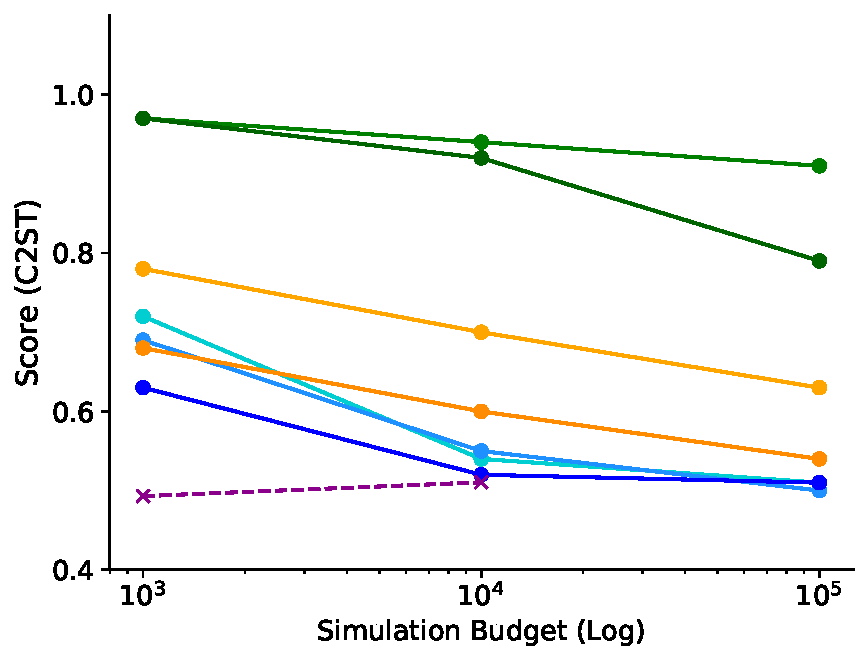
\includegraphics[width=.4\linewidth]{./figures/gaussian_linear_uniform.pdf}
%   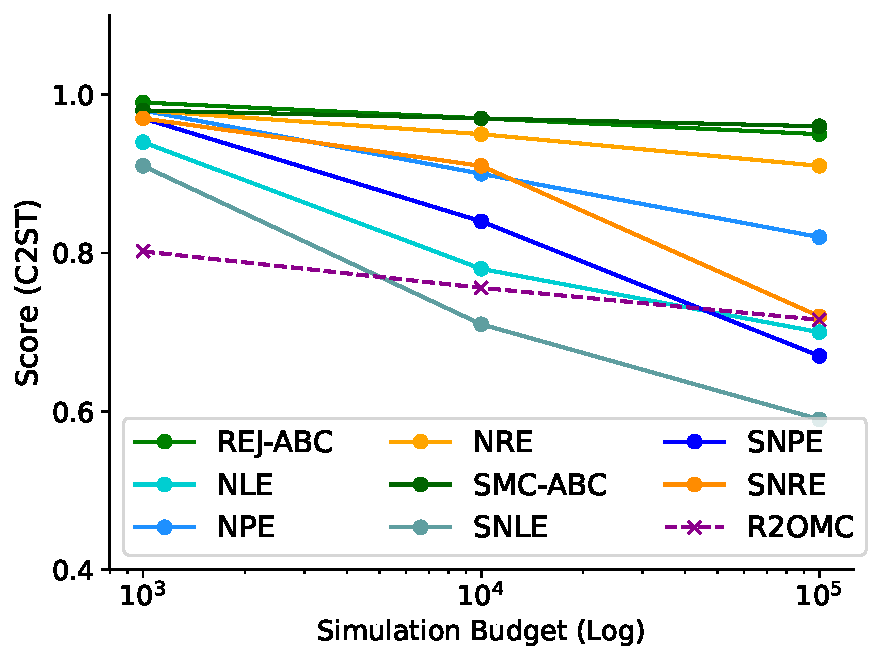
\includegraphics[width=.4\linewidth]{./figures/slcp.pdf}
%   \caption{Left---T.2: Gaussian Linear Uniform. Right---T.3: SLCP.}
%   \label{fig:exp_sbi_extra}
% \end{figure}

\subsection{MoG - Shifted Gaussian}

This additional experiment uses a simulator that samples from a mixture of two Gaussians, whose means are shifted by a constant value.

\begin{tabular}{@{}ll@{}}
  \textbf{Prior} & $\thb \sim \mathcal{U}(-15, 15)^4$ \\[5pt]
  \textbf{Simulator} & $\yb \sim \frac{1}{2} \left ( \mathcal{N}(\thb + \mathbf{5}, \mathbf{I}) + \mathcal{N}(\thb, \mathbf{I}) \right )$ \\[5pt]
  \textbf{Dimensionality} & $\thb \in \mathbb{R}^{4}$, $\yb \in \mathbb{R}^{4}$ \\[5pt]
\end{tabular}

We will use two separate cases: one with $N=4$ similar observations and another with $N=4$ different observations.
In both cases, the posterior is:
%
\begin{align}
  \label{eq:gauss_mult_obs}
  p(\thb|\{\data_n\}) &\propto p(\thb) p(\{\data_n\}|\thb) \\
                      &\propto p(\thb) \prod_{n=1}^{N} p(\data_n|\thb) \label{eq:gauss_mult_obs_1} \\
                      &\propto \mathcal{U}(-\mathbf{15},\mathbf{15}) \prod_{n=1}^{N} \dfrac{1}{2} \left ( \mathcal{N}(\data_n; \thb + \mathbf{5}, \mathbf{I}) + \mathcal{N}(\data_n; \thb, \mathbf{I}) \right ) \\
                      &\propto \mathcal{U}(-\mathbf{15},\mathbf{15}) \prod_{n=1}^{N} \dfrac{1}{2}\left ( \mathcal{N}(\thb; \data_n - \mathbf{5}, \mathbf{I}) + \mathcal{N}( \thb; \data_n, \mathbf{I}) \right ) \label{eq:gauss_mult_obs_3}\\
                      &\appropto \prod_{n=1}^{N} \left ( \mathcal{N}(\thb; \data_n - \mathbf{5}, \mathbf{I}) + \mathcal{N}( \thb; \data_n, \mathbf{I}) \right ) \label{eq:gauss_mult_obs_4}
\end{align}
In~(\ref{eq:gauss_mult_obs_1}), the factorization is due to the $N$ independently and identically distributed (iid) data points.
In~(\ref{eq:gauss_mult_obs_3}), we apply the property: $\mathcal{N}(\yb; \thb + \mub, \Sigma) = \mathcal{N}(\thb; \yb - \mub, \Sigma)$.
In~(\ref{eq:gauss_mult_obs_4}), we use that the data that we will use are sufficiently far from the boundaries so that we may ignore the boundary effects in the truncated distribution.

\paragraph{Case 1:}

In Case 1, we use $N=4$ similar observations: $\data_n \approx (0, \ldots, 0)$ for $n \in \{ 1, \ldots, N \}$. The ground-truth posterior is approximately:
%
\begin{equation}
  p(\thb | \data) \approx \mathcal{N}(\thb; - \mathbf{5}, \frac{1}{N} \mathbf{I}) + \mathcal{N}(\thb; \mathbf{0}, \frac{1}{N} \mathbf{I})
  \label{eq:mog_shifted_gaussian_case_1}
\end{equation}
%
\textbf{Proof.}
%
\begin{align} 
p(\thb|{\data_n}) 
&\appropto \prod_n^{N} \left ( \mathcal{N}(\thb; \data_n - \mathbf{5}, \mathbf{I}) + \mathcal{N}( \thb; \data_n, \mathbf{I}) \right ) \\
&\appropto \left( \mathcal{N}(\thb; - \mathbf{5}, \mathbf{I}) + \mathcal{N}(\thb; \mathbf{0}, \mathbf{I}) \right)^N \\
&\appropto \sum_{n=0}^N \binom{N}{n} (\mathcal{N}(\thb; - \mathbf{5}, \mathbf{I}))^n (\mathcal{N}(\thb; \mathbf{0}, \mathbf{I}))^{N-n} \\
&\appropto \left( \mathcal{N}(\thb; - \mathbf{5}, \mathbf{I}) \right)^N + \left( \mathcal{N}( \thb; \mathbf{0}, \mathbf{I}) \right)^N \label{eq:gauss_mult_obs_case_1_1}  \\
&\appropto \mathcal{N}(\thb; - \mathbf{5}, \frac{1}{N}\mathbf{I}) + \mathcal{N}( \thb; \mathbf{0}, \frac{1}{N}\mathbf{I}) \label{eq:gauss_mult_obs_case_1_2} 
\end{align}
%
In (\ref{eq:gauss_mult_obs_case_1_1}), for $n \in \{1, \ldots, N-1\}$ the terms involve products between 
$\mathcal{N}(\thb; - \mathbf{5}, \mathbf{I})$ and $ \mathcal{N}( \thb; \mathbf{0}, \mathbf{I})$ so they have 
a much smaller magnitude compared to $(\mathcal{N}(\thb; - \mathbf{5}, \mathbf{I}))^N$ ($n=N$) and $\mathcal{N}(( \thb; \mathbf{0}, \mathbf{I}))^N$ ($n=0$).
This allows us to approximate the expression by retaining only these two dominant terms.
In (\ref{eq:gauss_mult_obs_case_1_2}), we use the property that raising a Gaussian distribution to the power \(N\) results in a Gaussian with the same mean and a covariance scaled by \(\frac{1}{N}\). 
% In Figure~\ref{fig:multi_obs_case_1_gt} we show two dimensions, $\thb_i$ and $\thb_j$, of the ground truth posterior for $N=\{1, 4, 10, 20\}$ observations.

\paragraph{Case 2:}

In Case 2, we use an even number of $N$ observations that are split in two categories, 
half around $(0, \ldots, 0)$, i.e., 
$\data_n \approx (0, \ldots, 0)$ for $n \in \{ 1, \ldots, N/2 \}$ and the other half around 
$(5, \ldots, 5)$, i.e., 
$\data_n \approx (5, \ldots, 5)$ for $n \in \{ N/2 + 1, \ldots, N \}$.
The posterior, for values of $\thb$ sufficienty far from the boundary, is:
\begin{equation}
  p(\thb | \data) \approx \mathcal{N}(\thb; \mathbf{0}, \frac{1}{N} \mathbf{I})
  \label{eq:mog_shifted_gaussian_case_2}
\end{equation}

\textbf{Proof.}
\begin{align}
  p(\thb|\{\data_k\}) 
  &\appropto \prod_n^{N} \left ( \mathcal{N}(\thb; \data_n - \mathbf{5}, \mathbf{I}) + \mathcal{N}( \thb; \data_n, \mathbf{I}) \right ) \\
  &\appropto \prod_{n=1}^{N/2} \left ( \mathcal{N}(\thb; - \mathbf{5}, \mathbf{I}) + \mathcal{N}( \thb; \mathbf{0}, \mathbf{I}) \right ) \prod_{n=N/2 + 1}^{N} \left ( \mathcal{N}(\thb; \mathbf{0}, \mathbf{I}) + \mathcal{N}( \thb; \mathbf{5}, \mathbf{I}) \right )  \\
  &\appropto \prod_{n=1}^{N/2} \left ( \mathcal{N}(\thb; - \mathbf{5}, \mathbf{I}) + \mathcal{N}( \thb; \mathbf{0}, \mathbf{I}) \right ) \prod_{n=1}^{N/2} \left ( \mathcal{N}(\thb; \mathbf{0}, \mathbf{I}) + \mathcal{N}( \thb; \mathbf{5}, \mathbf{I}) \right )  \\
  &\appropto \left ( ( \mathcal{N}(\thb; - \mathbf{5}, \mathbf{I}) )^{N/2} + ( \mathcal{N}( \thb; \mathbf{0}, \mathbf{I}) )^{N/2} \right ) \left ( ( \mathcal{N}(\thb; \mathbf{0}, \mathbf{I}) )^{N/2} + ( \mathcal{N}( \thb; \mathbf{5}, \mathbf{I}) )^{N/2} \right ) \label{eq:gauss_mult_obs_case_2_1} \\
  &\appropto \mathcal{N}(\thb; \mathbf{0}, \mathbf{I})^N \label{eq:gauss_mult_obs_case_2_2} \\
  &\appropto \mathcal{N}( \thb; \mathbf{0}, \frac{1}{N}\mathbf{I}) \label{eq:gauss_mult_obs_case_2_3}
\end{align}
%
In (\ref{eq:gauss_mult_obs_case_2_1}), we keep only the dominant terms, as in Case 1.
In (\ref{eq:gauss_mult_obs_case_2_2}), we use that terms that involve combinations of \(\mathcal{N}(\thb; \mathbf{0}, \mathbf{I})^{N/2}\), \(\mathcal{N}(\thb; -\mathbf{5}, \mathbf{I})^{N/2}\) and \(\mathcal{N}(\thb; \mathbf{5}, \mathbf{I})^{N/2}\) have significantly smaller magnitudes compared to the dominant ones; \(\mathcal{N}(\thb; \mathbf{0}, \mathbf{I})^{N/2} \mathcal{N}(\thb; \mathbf{0}, \mathbf{I})^{N/2}\).
In (\ref{eq:gauss_mult_obs_case_2_3}), we use the property that raising a Gaussian distribution to the power \(N\) results in a Gaussian with the same mean and a covariance scaled by \(\frac{1}{N}\).
% In Figure~\ref{fig:multi_obs_case_2_gt} we show two dimensions, $\thb_i$ and $\thb_j$, of the ground truth posterior for $N=\{1, 4, 10, 20\}$ observations.

\paragraph{Results.}

Figure~\ref{fig:multi_obs} demonstrates that \rromc~aligns closely with the ground truth posterior, correctly capturing the two modes in Case 1 and the single mode in Case 2.
% Due to the approximation error introduced by $\epsilon$, \rromc~exhibits a slightly higher variance compared to the ground truth.
In contrast, both \romc~struggles with multiple observations, resulting in their samples being distributed along the \(45^{\circ}\) line.

\begin{figure}
    \centering
    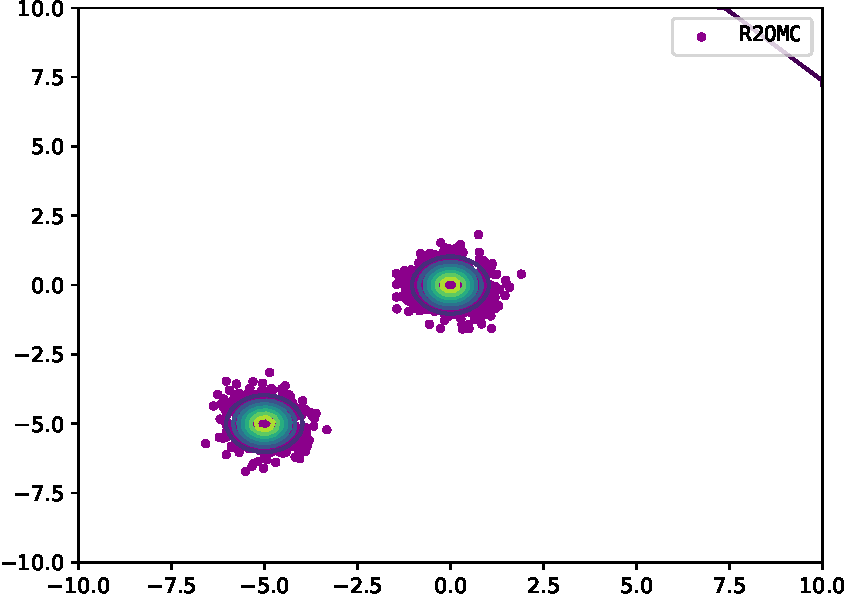
\includegraphics[width=0.23\linewidth]{figures/old/multi_obs_case_1_iterative_romc}
    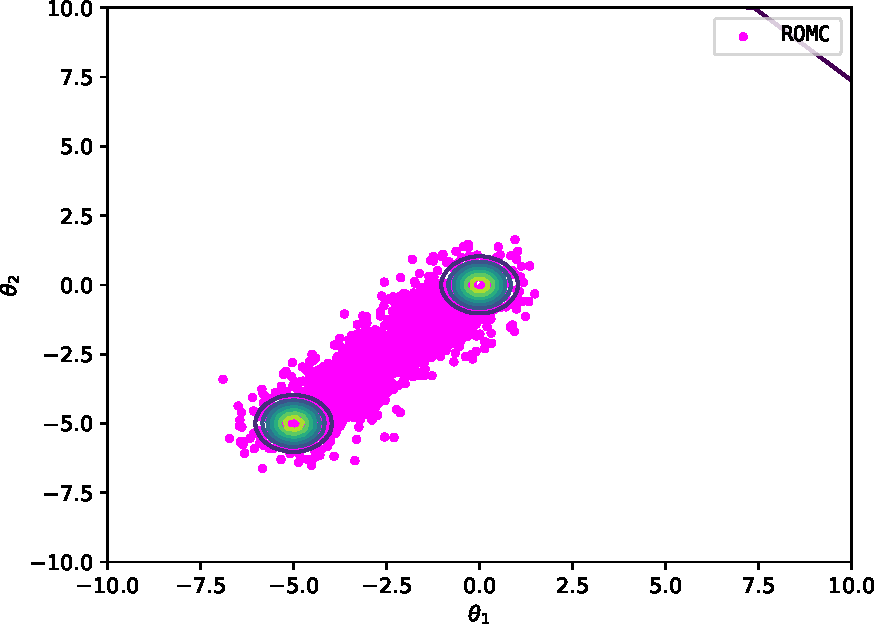
\includegraphics[width=0.23\linewidth]{figures/old/multi_obs_case_1_romc}
    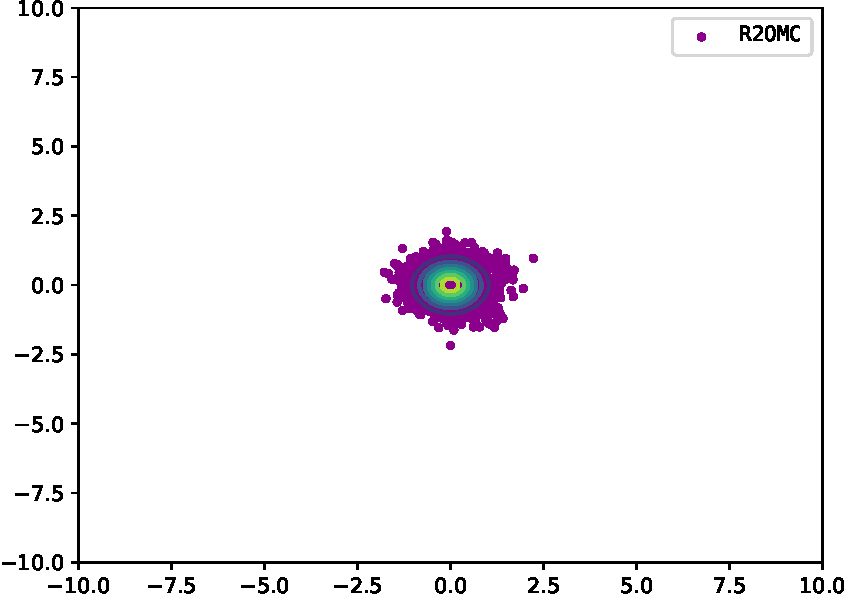
\includegraphics[width=0.23\linewidth]{figures/old/multi_obs_case_2_iterative_romc}
    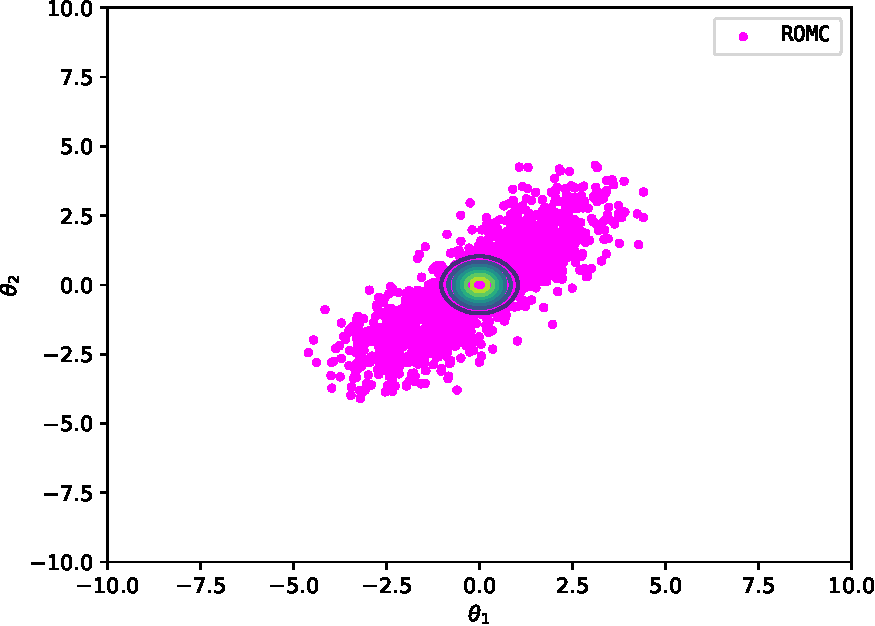
\includegraphics[width=0.23\linewidth]{figures/old/multi_obs_case_2_romc}
    \caption{From left to right: R2OMC on Case 1, Naive-ROMC on Case 1, R2OMC on Case 2, and Naive-ROMC on Case 2.}
    \label{fig:multi_obs}
\end{figure}